\chapter{روش‌ها و مجموعه‌داده}
\section{بررسی آماری مجموعه داده}

در این پژوهش از مجموعه داده
\lr{PhysioNet}\cite{physionet_hssayeni2020intracranial,hssayeni2020computed}
استفاده شده است که شامل حاشیه‌نویسی برای وظیفه طبقه‌بندی و قطعه‌بندی است. این مجموعه داده  شامل مجموعه‌ای از سی‌تی‌اسکن‌های مغزی است که به صورت عمومی در دسترس است.
\begin{figure}[h]
\centering
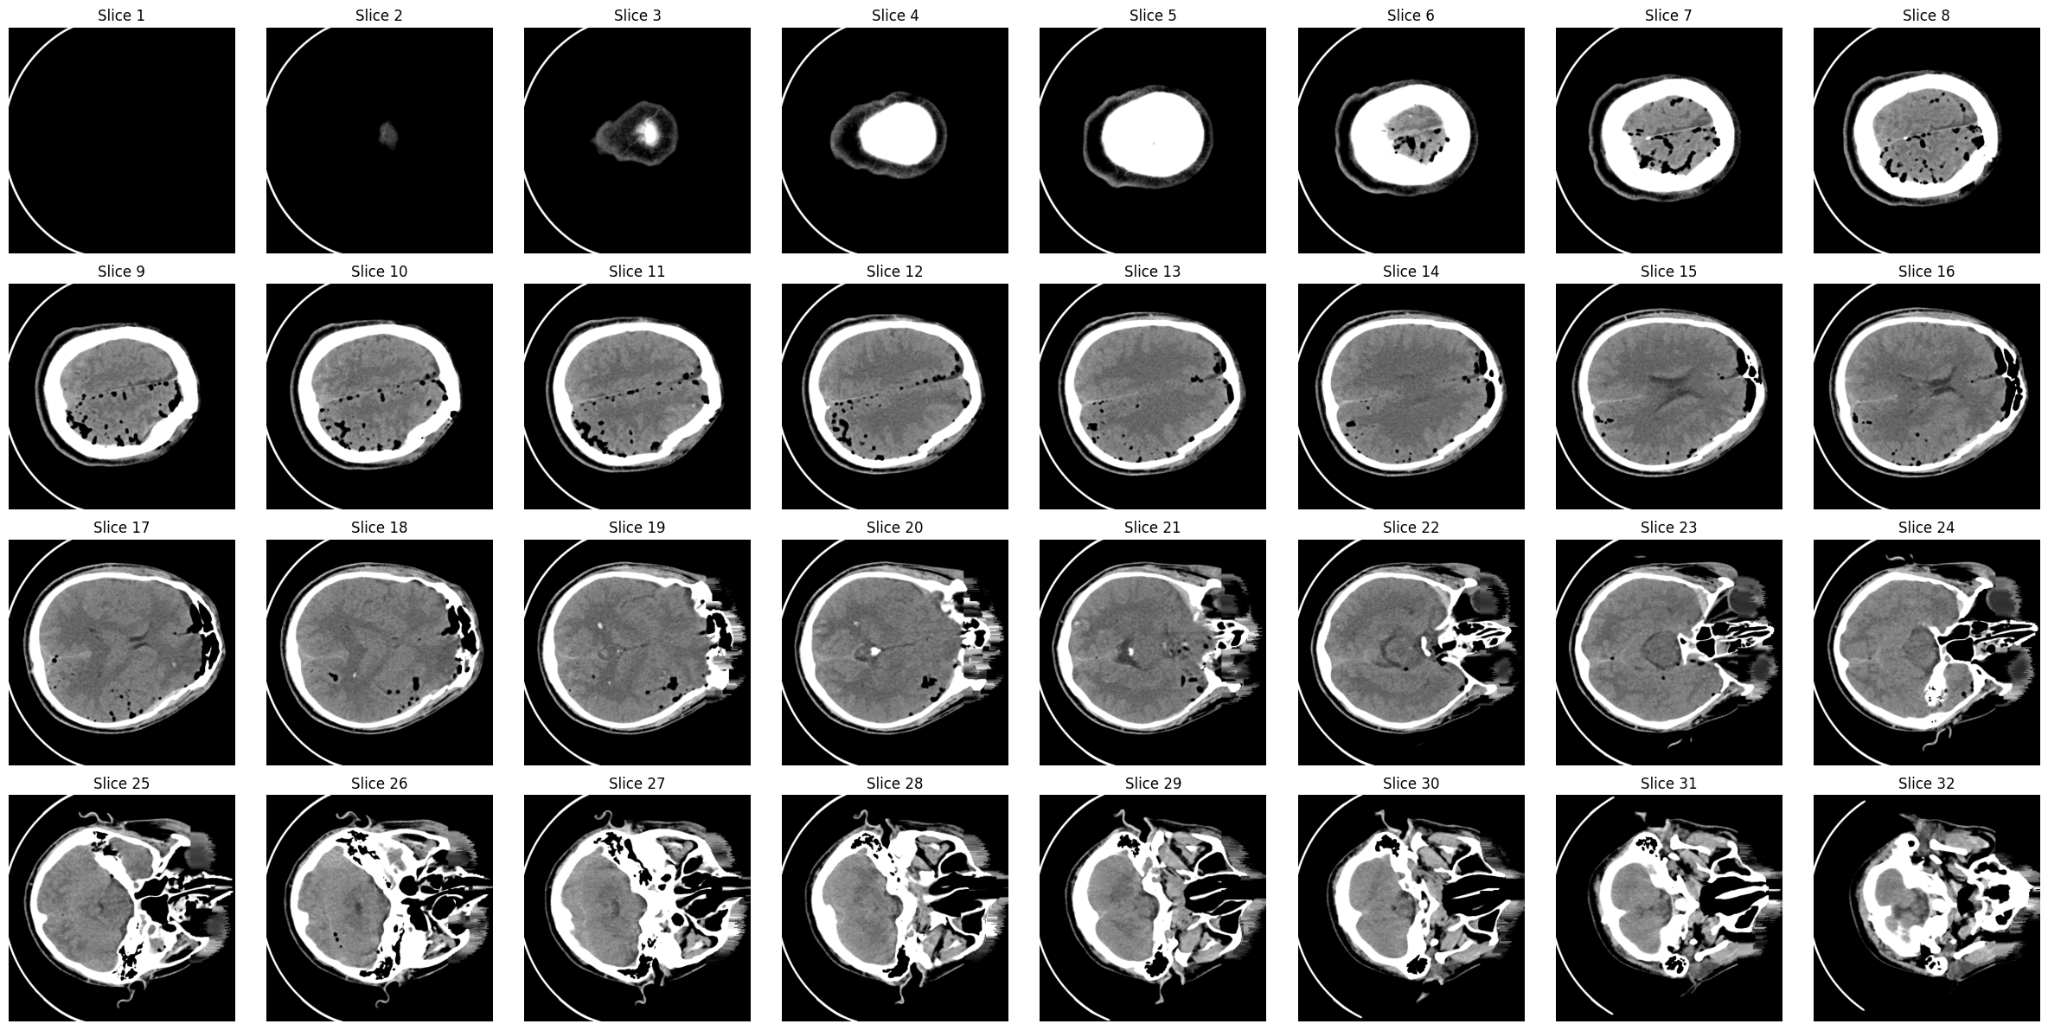
\includegraphics[width=1.0\linewidth]{Images/Chapter2/3d}
\caption{یک نمونه کامل از تصاویر سی‌تی‌اسکن}
\label{fig:ct2-3d}
\end{figure}


همانطور که در 
\autoref{fig:ct2-3d}
نمایش‌داده‌شده است، سی‌تی‌اسکن یک نوع تصویر سه‌بعدی است که از برش‌های دو بعدی تشکیل شده است. 
\autoref{fig:read-ct}
 نشان می‌دهد که
 با توجه به جهت بررسی برش‌های سی‌تی‌اسکن، این تصاویر به سه دسته 
 \lr{Axial}, \lr{Sagital} و \lr{Coronal}
 تقسیم می‌شوند.
\begin{figure}[h]
\centering
\includegraphics[width=1.0\linewidth]{"Images/Chapter2/read CT"}
\caption{خوانش‌های متفاوت از تصاویر سی‌تی‌اسکن
\cite{kaggleCTScansDICOM}}
\label{fig:read-ct}
\end{figure}
 
مجموعه‌داده 
\lr{PhysioNet}
 شامل 82 سی‌تی‌اسکن با برش‌‌های 
\lr{Axial}
است که بین فوریه و آگوست 2018 از بیمارستان آموزشی 
\lr{Al Hilla }
 در عراق جمع‌آوری شده است. این اسکن‌ها شامل طیف وسیعی از بیماران هستند که از یک روز تا 72 سال سن دارند و میانگین سن آنها 
 $27.8 \pm 19.5$
 سال است. تنوع سنی این مجموعه داده بر مقیاس، شکل جمجمه و بافت مغز در سی‌تی‌اسکن تأثیر می‌گذارد، عاملی که می‌تواند عملکرد مدل‌های یادگیری عمیق برای تشخیص و قطعه‌بندی خونریزی درون جمجمه‌ای را تحت تأثیر قرار دهد. توزیع جنسیت در ای نمجموعه‌داده به گونه‌ای است که 56\%  بیماران مرد و 44\% آنها زن هستند.
82 بیماری که در این مجموعه داده وجود دارد که 7 مورد از آنها طی قرایند حاشیه‌نویسی گم شده‌اند و از بین 75 بیمار موجود، 36 نفر دارای خونریزی درون‌جمجمه‌ای تشخیص داده شدند.
\autoref{fig:ch2-slice-number}
نمودار مروبط به تعداد برش‌های هر بیمار در این مجمموعه‌داده است؛ تصاویر سی‌تی‌اسکن موجود در این مجموعه داده،  به طور متوسط شامل 34 برش با ضخامت برش 5 میلی‌متر دارند و در مجموع 2814 برش در این مجموعه‌داده وجود دارد. 
\begin{figure}[h]
\centering
\includegraphics[width=1.0\linewidth]{"Images/Chapter2/Slice number"}
\caption{‌تعداد برش‌های بیماران بر اساس شناسه اختصاصی آنها}
\label{fig:ch2-slice-number}
\end{figure}

با این حال، این مجموعه داده به دلیل عدم توازن در سطح برش شناخته می‌شود، زیرا تنها 318 برش دارای خونریزی هستند در حالی که بقیه 2496 برش سالم هستند. در این مجموعه داده، 24 برش شامل زیرگروه
 \lr{IVH}،
  73 برش شامل زیرگروه
 \lr{CPH}، 
  18 برش شامل زیرگروه
 \lr{SDH}،
173 برش شامل زیرگروه
 \lr{EDH} 
 و 56 برش شامل زیرگروه 
 \lr{SDH}
هستند. با توجه به تفاوت شکل انواع زیرگروه‌های خونریزی و محل وقوع آنها، این ارقام نشان دهنده عدم وجود تعداد برش کافی برای بعضی از انواع زیرگروه‌های است.
در این مجموعه‌داده، برش‌های سی‌تی‌اسکن توسط دو پرتوشناس بررسی شده‌است و هر برش سی‌تی‌اسکن از نظر وجود خونریزی یا شکستگی توسط آنها بررسی و برچسب‌گذاری شده است. در ادامه سی‌تی‌اسکن‌های دو بیمار، به علت کیفیت ضعیف تصاویر و به توصیه پرتوشناس‌ها حذف شدند\cite{kyung2022improved}.

\autoref{fig: ch2-distribution}
نمودارهای توزیع بیمارمحور و برش‌محور مجموعه‌داده را نمایش می‌دهد؛ همانطور که از ‎\autoref{fig: ch2-patient distrbiution}‎ مشخص است در بررسی بیمار‌محور این مجموعه‌داده، عدم توازن دیده نمی‌شود اما در بررسی برش‌محور، همانطور که در ‎\autoref{fig: ch2-slice distribution}‎ 
مشخص است، عدم توازن شدیدی در تعداد برش‌های دارای خونریزی وجود دارد که این مسئله آموزش مدل‌های شبکه عصبی را با چالش مواجه می‌کند.
 \begin{figure}[ht]
		\centering % <-- added
		\begin{subfigure}{0.45\textwidth}
			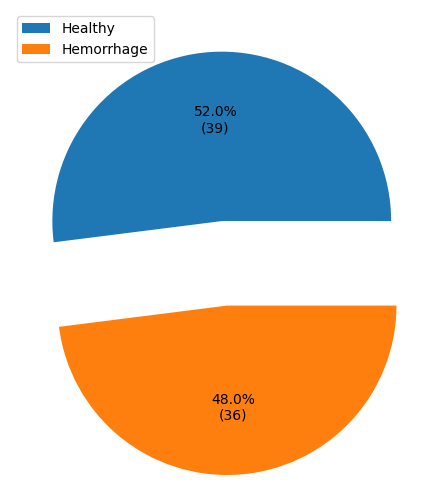
\includegraphics[width=\linewidth]{Images/Chapter2/patient distrbiution.png}
			\caption{}
			\label{fig: ch2-patient distrbiution}
		\end{subfigure}\hfil % <-- added
		\begin{subfigure}{0.45\textwidth}
			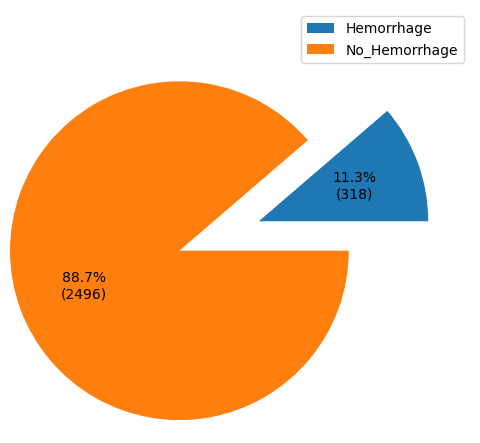
\includegraphics[width=\linewidth,]{Images/Chapter2/slice distribution.png}
			\caption{}
			\label{fig: ch2-slice distribution}
		\end{subfigure}
		\caption{توزیع بیماران و برش‌ها در مجموعه داده 
		\lr{PhysioNet}}
		\label{fig: ch2-distribution}
\end{figure} 

 علاوه بر وجود عدم توازن در حالت برش‌محور، عدم توازن شدیدی در قطعه‌بندی نواحی دارای خونریزی نسبت به نواحی سالم در برش‌های دارای خونریزی وجود دارد که به موجب آن در یک تصویر با ابعاد
$512\times512$،
به صورت میانگین نزدیک به 2000 پیکسل
\LTRfootnote{Pixel}
دارای خونریزی درون‌جمجمه‌ای وجود دارد که این مسئله آموزش مدل‌های شبکه عصبی را به منظور وظیفه قطعه‌بندی با چالش بسیار جدی مواجه می‌کند. 
\autoref{fig: ch2-slice hist}
نشان‌دهنده توزیع نرمال‌شده 
\LTRfootnote{Normalized}
مقدار پیکسل‌های برش‌های سالم و برش‌های دارای خونریزی می‌باشد، با توجه به
\autoref{fig: ch2-slice hist whole}، 
اکثر پیکسل‌های تصاویر مقداری نزدیک به 
$-1000$
و نقطه بیشینه محلی بعدی برای این نمودار توزیع، در نزدیک مقادیر 30 می‌باشد که این مقادیر به نسبت پیکسل‌ها با مقادیر نزدیک به 
$-1000$
خیلی کمتر می‌باشد.


 \begin{figure}[ht]
		\centering % <-- added
		\begin{subfigure}{0.45\textwidth}
			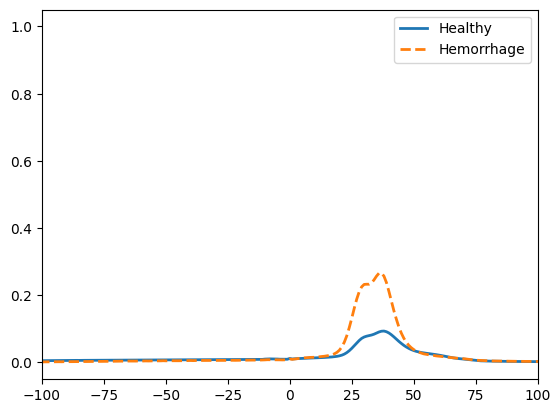
\includegraphics[width=\linewidth]{Images/Chapter2/Pixel histogram.png}
			\caption{}
			\label{fig: ch2-slice hist whole}
		\end{subfigure}\hfil % <-- added
		\begin{subfigure}{0.45\textwidth}
			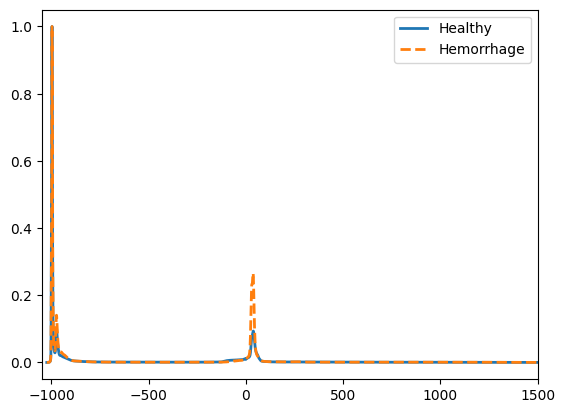
\includegraphics[width=\linewidth,]{Images/Chapter2/Pixel histogram lim.png}
			\caption{}
			\label{fig: ch2-slice hist lim}
		\end{subfigure}
		\caption{توزیع پیکسلی برش‌ها برای برش‌های دارای خونریزی در مقال برش‌های سالم}
		\label{fig: ch2-slice hist}
\end{figure} 

\autoref{fig:ch2-pixel-hist-ich-vs-healthy}
نمایش‌دهنده توزیع پیکسل‌های دارای خونریزی و تمام پیکسل‌های تصاویر رادیوگرافی می‌باشد که در محدوده بین 
$-100$
تا 
$100$
واقع شده است و نسبت به مقادیر همین بازه نرمال گشته است. همانطور که از این دو نمودار مشخص است، مقادیر مربوط به ضایعه خونریزی،‌مقادر کمی از مقادیر بقیه بافت‌های مغز روشن‌تر است اما همپوشانی این دو نمودار نشان می‌دهد که تشخیص خونریزی درون‌جمجمه‌ای تنها با استفاده از مقدار پیکسلی آن بسیار دشوار می‌باشد و نیاز هست تا از شبکه‌هایی استفاده شود تا به اشکال موجود در تصویر نیز حساسیت داشته باشند.


\begin{figure}[h]
\centering
\includegraphics[width=1.0\linewidth]{"Images/Chapter2/pixel hist ich vs healthy"}
\caption{توزیع نرمال‌شده پیکسل‌های دارای خونریزی درمقابل تمام پیکسل‌های تصاویر}
\label{fig:ch2-pixel-hist-ich-vs-healthy}
\end{figure}


\autoref{fig:ch2-slice-number}
توزیع خونریزی درون‌جمجمه‌ای را بر اساس شماره برش در تصویر سی‌تی‌اسکن نشان می‌دهد که بر اساس آن مشخص است به ازای بعضی از شماره برش‌ها، خونریزی درون‌جمجمه‌ای وجود ندارد و این برش‌ها از اهمیت کمتری برای مدل‌های یادگیری ماشین برخوردار هستند.

\begin{figure}[h]
\centering
\includegraphics[width=1.0\linewidth]{"Images/Chapter2/slice hist"}
\caption{توزیع خونریزی بر اساس برش‌ها}
\label{fig:ch2-slice-hist}
\end{figure}


باتوجه به مطالبی که دی این بخش مطرح شد،‌می‌توان نتیجه‌ گرفت که مجموعه داده
 \lr{PhysioNet}،
به عنوان تنها مجموعه‌داده عمومی قطعه‌بندی خونریزی درون‌جمجمه‌ای، می‌تواند یک مجموعه‌داده معیار برای بررسی عملکرد مدل‌های پردازش تصویر باشد. 

\autoref{fig:ch3-wholeheatmap}
نمایش پراکندگی مکانی خونریزی درون‌جمجمه‌ای را نشان می‌دهد که در مجموعه‌داده
\lr{PysioNet}
وجود دارد. این پراکندگی نشان می‌دهد که خونریزی درون‌جمجمه‌ای تنها در قسمت‌های خاصی از برش‌های سی‌تی‌اسکن اتفاق می‌افتد و از طرف دیگر احتمال وجوذ خونریزی در اطراف جمجمه و ناحیه شقیقه،‌ بیشتر از پیشانی و پشت سر می‌باشد.
\autoref{fig:heatmaps}
نمایش زیرمجموعه‌های متفاوتی است که در فرایند آموزش و ارزیابی مدل دخیل بوده‌اند. باید توجه داشت که در این تصویر، نقشه پراکندگی مربوط‌ به هر 
\lr{Fold}
نشان‌دهنده زیرمجموعه آموزش به‌ازای آن 
\lr{Fold}
است.  
\begin{figure}[h]
\centering
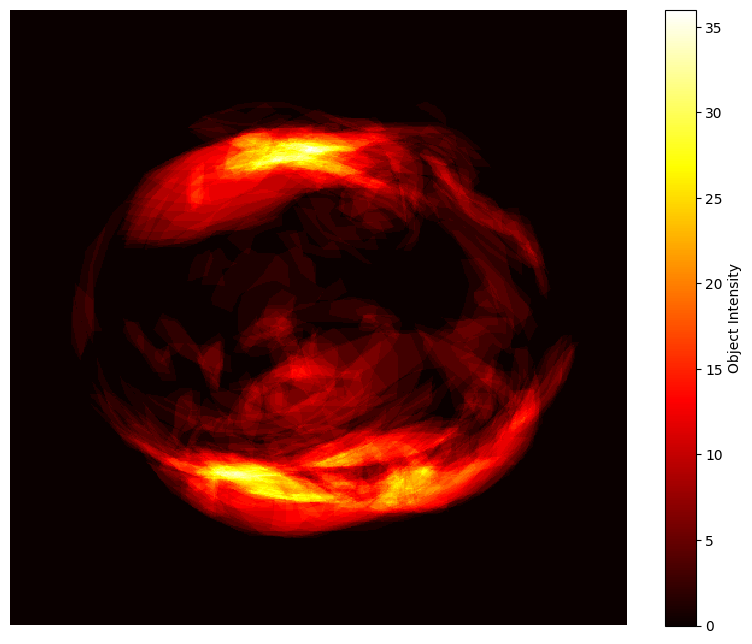
\includegraphics[width=1.0\linewidth]{Images/Chapter2/whole_heatmap}
\caption{ پراکندگی مکانی خونریزی در مجموعه‌داد
\lr{PhysioNet}}
\label{fig:ch3-wholeheatmap}
\end{figure}


\begin{figure}[h!]
    \centering % Center the figure
    \begin{subfigure}{0.33\textwidth}
        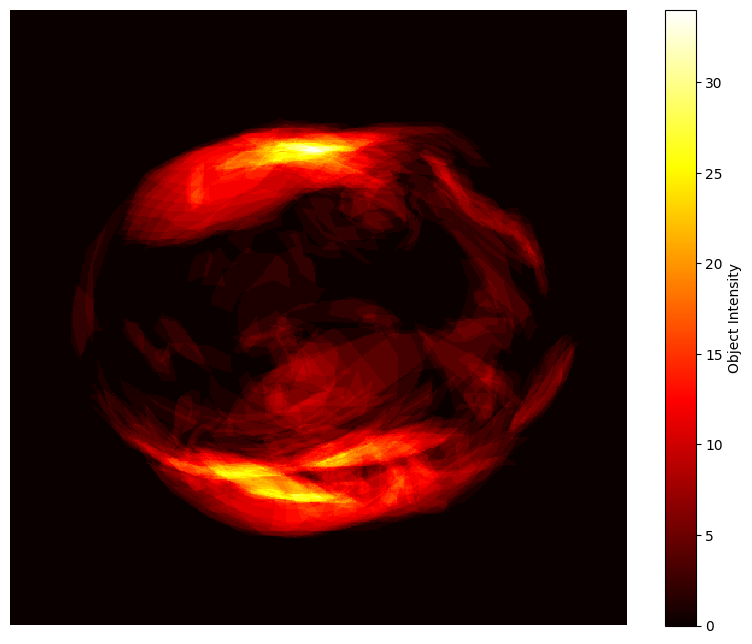
\includegraphics[width=\linewidth]{Images/chapter2/fold0_heatmap.png}
        \caption{\lr{Fold 0}}
        \label{fig:fold0}
    \end{subfigure}\hfil % Space between images
    \begin{subfigure}{0.33\textwidth}
        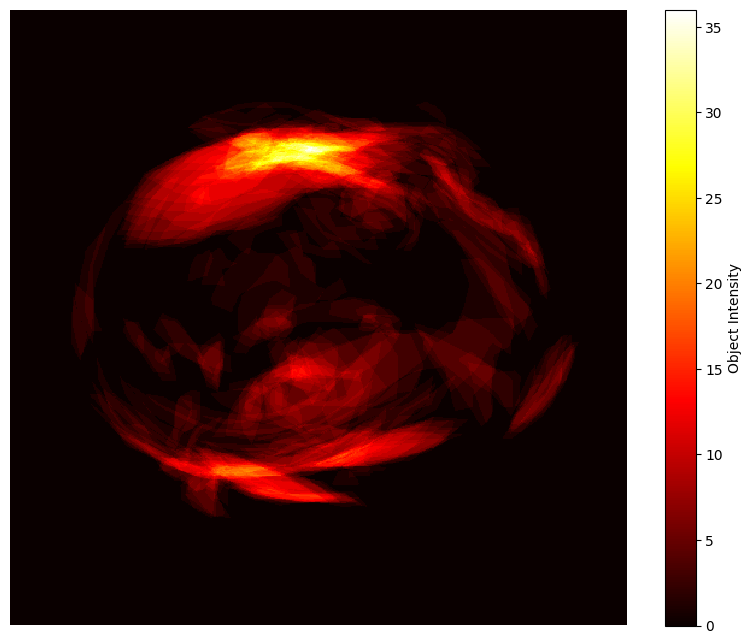
\includegraphics[width=\linewidth]{Images/chapter2/fold1_heatmap.png}
        \caption{\lr{Fold 1}}
        \label{fig:fold1}
    \end{subfigure}\hfil
    \begin{subfigure}{0.33\textwidth}
        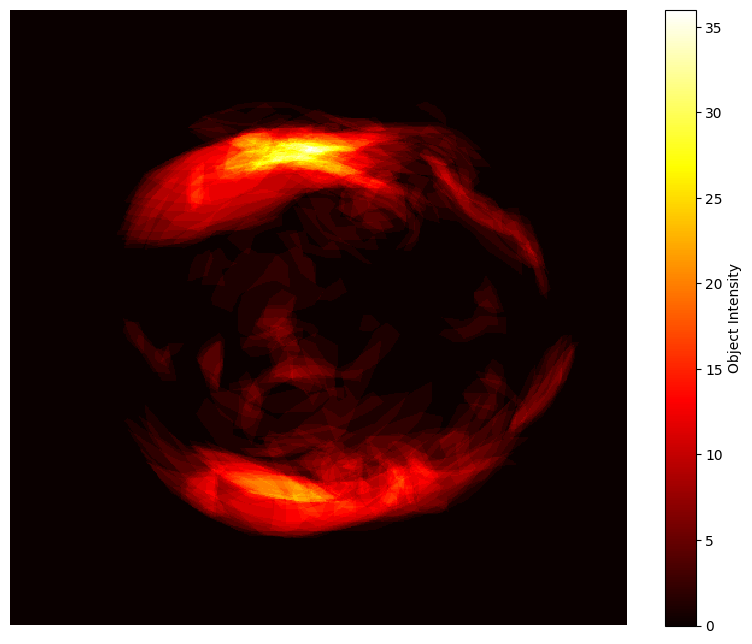
\includegraphics[width=\linewidth]{Images/chapter2/fold2_heatmap.png}
        \caption{\lr{Fold 2}}
        \label{fig:fold2}
    \end{subfigure}

    \vspace{1em} % Add vertical space between rows

    \begin{subfigure}{0.33\textwidth}
        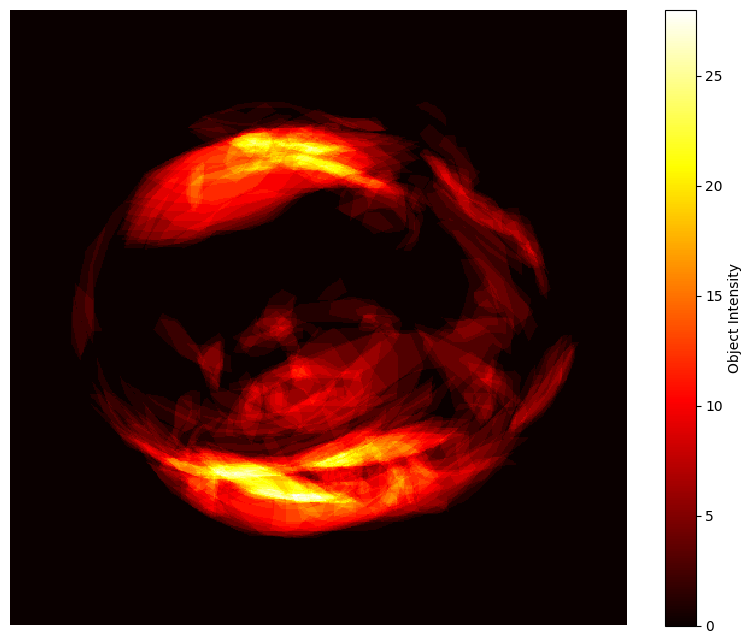
\includegraphics[width=\linewidth]{Images/chapter2/fold3_heatmap.png}
        \caption{\lr{Fold 3}}
        \label{fig:fold3}
    \end{subfigure}\hfil
    \begin{subfigure}{0.33\textwidth}
        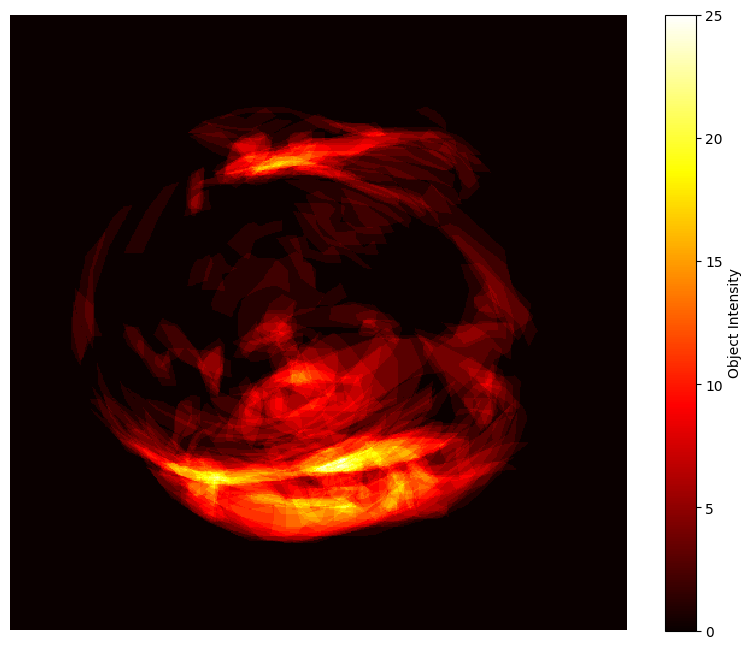
\includegraphics[width=\linewidth]{Images/chapter2/fold4_heatmap.png}
        \caption{\lr{Fold 4}}
        \label{fig:fold4}
    \end{subfigure}\hfil
    \begin{subfigure}{0.33\textwidth}
        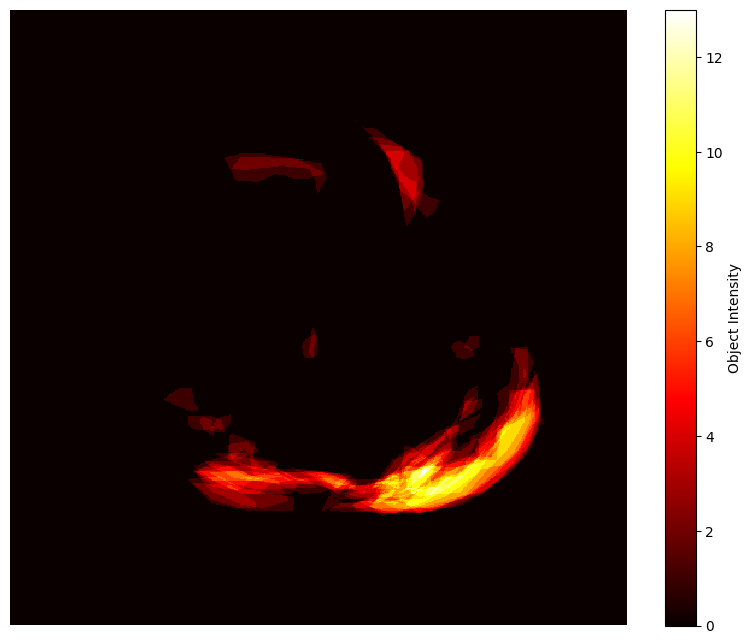
\includegraphics[width=\linewidth]{Images/chapter2/test_heatmap.png}
        \caption{مجموعه ارزیابی}
        \label{fig:test}
    \end{subfigure}

    \caption{پراکندگی مکانی خونریزی در زیرمجموعه‌های متفاوت از مجموعه‌داده}
    \label{fig:heatmaps}
\end{figure}


\section{پیش‌پردازش\protect\LTRfootnote{Pre-process}}

در تصاویر پرتونگاری سی‌تی‌اسکن، از اشعه ایکس
\LTRfootnote{X-Ray}
 به منظور ثبت تصویر اندام درونی بدن استفاده می‌شود. در این روش،‌یک کاتد
 \LTRfootnote{Cathode}
را برانگیخته می‌کنند تا الکترون‌های
 \LTRfootnote{Electron}
 پرانرژی را آزاد ‌کند. با آزاد شدن الکترون‌ها، انرژی به صورت اشعه ایکس آزاد می‌شود و اشعه ایکس از بافت‌ها عبور کرده و به آشکارساز در سمت دیگر برخورد می‌کند. هرچه بافت متراکم‌تر باشد، اشعه ایکس بیشتری را جذب می‌کند؛ مثلا باقت استخوانی به علت تراکم بالا،‌ اشعه ایکس بیشتری جذب می‌کند و در نتیجه آن اشعه کمتری به آشکارساز می‌رسد که موجب سفید شدن آن قسمت از تصویر خواهد شد اما این مسئله درمورد هوا برعکس است
 \cite{kaggleCTScansDICOM}.
در مقایسه با تصویر اشعه ایکس ساده، سی‌تی‌اسکن دارای تفکیک‌پذیری بیشتر است و هیچ هم‌پوشانی در ساختارها وجود ندارد.
دستگاه‌های سی‌تی‌اسکن که از کالیبراسیون
\LTRfootnote{Calibration}
 درستی برخوردار باشند، تصاویر خود را طبق یکای 
 \lr{Hounsfield}
ثبت می‌کنند. این یکا به پرتونگارها و محققین اجازه می‌دهد تا بتوانند با آستانه گذاری مناسب، جزییات بافت هدف خود را در تصویر رویت‌پذیرتر کنند. تصاویر سی‌تی‌اسکن به صورت معمول بر اساس یکای
\lr{Hounsfield}
 مقادیر پیکسلی بین $-1024$ تا 3000 را دارا می‌باشند.

\autoref{fig:ch2-hu}
نشان‌دهنده مقدار پیکسلی است که هر بافت در تصویر سی‌تی‌اسکن از خود نشان می‌دهد. پروتونگارها،‌ پزشک‌ها و محققین برای اینکه بتوانند یک بیماری خاص را مورد بررسی قرار بدهند، برش‌های تصاویر را در بازه‌های خاصی از یکای
\lr{Hounsfield}
مورد بررسی قرار می‌دهند که به این نوع از پیش‌پردازش تصاویر سی‌تی‌اسکن،‌پنجره‌گذاری
\LTRfootnote{Windowing}
می‌گویند. 
\begin{figure}[H]
\centering
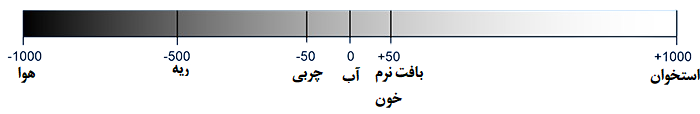
\includegraphics[width=1.0\linewidth]{Images/Chapter2/HU}
\caption{اثر بافت‌های متفاوت در یکای
 \lr{Hounsfield}
 \cite{kaggleCTScansDICOM}}
\label{fig:ch2-hu}
\end{figure}

در روش پنجره‌گذاری، دو مقدار مرکز پنجره
\lr{(WC)}
و پهنای پنجره
\lr{(WW)}
بازه هدف را در تصویر مشخص می‌کند و به موجب آن هر پیکسل که مقدار آن از حداقل بازه کمتر باشد، مقدارش برابر با حداقل بازه می‌شود و هر پیکسل که مقدارش از حداکثر بازه بیشتر باشد، مقدارش برابر حداکثر بازه می‌شود. ‎
\autoref{code:ch2-windowing}
روش اعمال پنجره‌گذاری روی تصاویر را نمایش می‌دهد که در آن 
\lr{Normalize}
به منظور انتقال مقادیر تصویر بعد از پنجره‌گذاری بین 0 و 1 است و 
\lr{Threshold}
تابعی است که در اثر آن مقادیر کمتر از حداقل بازه هدف به مقدار خداقل تغییر پیدا می‌کنند و مقادیری بیشتر از حداکثر بازه به مقدار حداکثر تبدیل می‌شوند.   
\begin{latin}
\begin{equation}
\text{Processed Image} = \text{Normalize}(\text{Threshold}(\text{Image}, WC-\frac{WW}{2},WC+\frac{WW}{2})) 
\end{equation}
\label{code:ch2-windowing}
\end{latin}

پرتونگار‌ها مقادیر مشخصی را برای شناسایی انواع مختلف اندام در تصاویر سی‌تی‌اسکن تعیین کرده‌اند به عنوان مثال، در مجموعه‌داده
\lr{‌PhysioNet}،
پردازش تصویر اصلی به‌ازای مرکز پنجره 40 و پهنای پنجره 120، پنجره مغز استخراج می‌شود و به‌ازای مرکز پنجره 700 و پهنای پنجره 3200،‌ پنجره استخوان استخراج می‌شود.
\autoref{fig:ch2-windowed-ct-sample}
اثر پنجره‌گذاری را بر یک نمونه برش سی‌تی‌اسکن نشان می‌دهد. همانطور که از این
\autoref{fig:ch2-before-processing}
 مشخص است، تصویر قبل از پیش‌پردازش جزییات خاصی را به ما نشان نمی‌دهد و اگر این تصویر را بدون نرمال کردن برای آموزش شبکه‌عصبی استفاده کنیم، باعث می‌شود که لایه‌های ابتدایی شبکه مقادیر خیلی بزرگی را ایجاد کنند و در نتیجه عملکرد مدل کاهش پیدا بکند و اگر این تصویر را نرمال کنیم، به علت بازه بسیار زیاد یکای 
\lr{Hounsfield}
تفکیک‌پذیری مقادیر تصویر به شدت کاهش پیدا می‌کند. در ادامه
\autoref{fig:ch2-brain-window}, \autoref{fig:ch2-bone-window} و \autoref{fig:ch2-subdural-window}
اثر سه پنجره مرسوم مغز، استخوان و سابدورال را مشاهده می‌کنیم که هرکدام تفکیک‌پذیری بافت هدف خود را افزایش داده‌اند و در پنجره مغز و سابدورال، محل خونریزی به وضوح مشخص است.
\autoref{fig:ch2-selected-window}
 پنجره انتخابی را نشان می‌دهد که براساس محدوده موجود در  
\autoref{fig:ch2-pixel-hist-ich-vs-healthy}
انتخاب شده‌است و در نتیجه آن، محل خونریزی بروز بیشتری پیدا کرده است. در ادامه این پژوهش،‌ پنجره مغز به عنوان پنجره اصلی آموزش و ارزیابی مدل‌ها درنظر گرفته شده است.

از دیگر روش‌های پیش‌پردازشی که در این پروژه استفاده شده است، افزایش مصنوعی داده می‌باشد که به جهت بهبود عملکرد مدل در فرایند آموزش انجام شده است. تبدیل‌های افزایش مصنوعی داده‌ای که در این پژوهش استفاده شده است شامل چرخش، برش تصادفی،‌ تبدیل آیینه حول محور افقی و‌ بزرگ‌نمایی تصادفی است. به علت اینکه سر تمامی بیماران در مجموعه‌داده 
\lr{PhysioNet}
جهت یکسانی دارد، استفاده از تبدیل آیینه حول محور عمودی باعث ایجاد تصاویری می‌شود که معادل آنها در مجموعه‌داده وجود ندارد
\cite{hssayeni2020intracranial}.



\begin{figure}[h!]
    \centering % <-- added
    \begin{subfigure}{0.33\textwidth}
      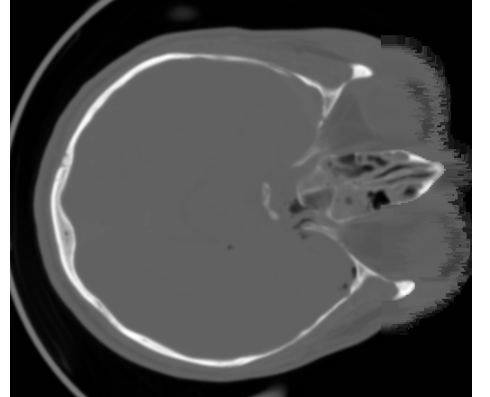
\includegraphics[width=\linewidth]{Images/chapter2/before_processing_no_caption.png}
      \caption{قبل از پردازش}
      \label{fig:ch2-before-processing}
    \end{subfigure}\hfil % <-- 
    \begin{subfigure}{0.33\textwidth}
      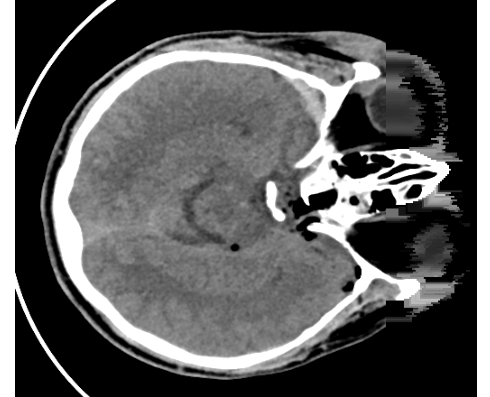
\includegraphics[width=\linewidth]{Images/chapter2/brain_window_no_caption.png}
      \caption{پنجره مغز}
      \label{fig:ch2-brain-window}
    \end{subfigure}\hfil % <-- 
    \begin{subfigure}{0.33\textwidth}
      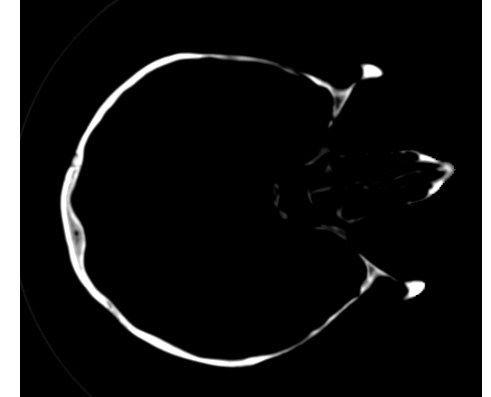
\includegraphics[width=\linewidth]{Images/chapter2/bone_window_no_caption.png}
      \caption{پنجره استخوان}
      \label{fig:ch2-bone-window}
    \end{subfigure}\hfil % <-- 
    \begin{subfigure}{0.33\textwidth}
      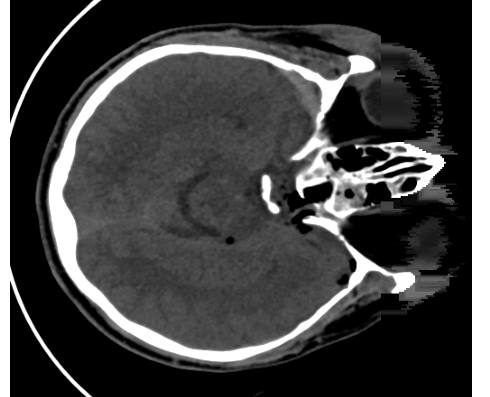
\includegraphics[width=\linewidth]{Images/chapter2/subdural_window_no_caption.png}
      \caption{پنجره ساب‌دورال}
      \label{fig:ch2-subdural-window}
    \end{subfigure}\hfil % <-- 
    \begin{subfigure}{0.33\textwidth}
      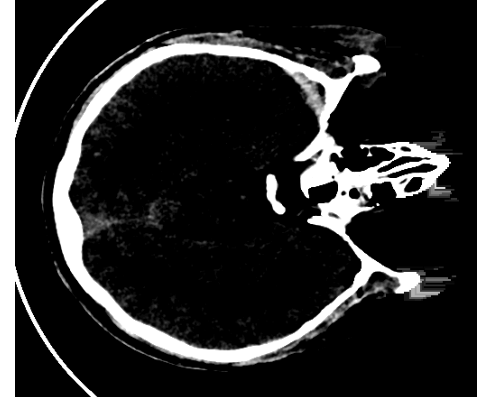
\includegraphics[width=\linewidth]{Images/chapter2/selected_window_no_caption.png}
      \caption{پنجره انتخابی}
      \label{fig:ch2-selected-window}
    \end{subfigure}\hfil % <-- 
    \begin{subfigure}{0.33\textwidth}
      
\includegraphics[width=\linewidth]{Images/chapter2/bleed_location_no_caption.png}
      \caption{محل خونریزی}
      \label{fig:ch2-bleed-location}
    \end{subfigure}
\caption{تاثیر اثر پنجره‌گذاری در نمایش خونریزی در یک برش از سی‌تی‌اسکن}
\label{fig:ch2-windowed-ct-sample}
\end{figure}

\section{روش پردازش تصاویر}
شبکه‌های عصبی عمیق به عنوان یکی از روش‌های محبوب در حوزه‌ی یادگیری ماشین شناخته می‌شوند. این شبکه‌ها از ساختارهایی شبیه به مغز انسان تشکیل شده‌اند که شامل تعدادی نورون \LTRfootnote{Neuron} مصنوعی هستند و قادرند با استفاده از داده‌های ورودی، الگوها و روابط پیچیده را بیاموزند. یادگیری عمیق، شاخه‌ای از شبکه‌های عصبی است که با افزایش تعداد لایه‌های مخفی در شبکه، امکان پردازش و تحلیل داده‌های بسیار پیچیده و بزرگ را فراهم می‌کند.
در این پژوهش، روش اصلی مورد استفاده برای پردازش کامپیوتری تصاویر، یادگیری عمیق است.
\subsection{یادگیری عمیق و اصول اولیه}
یادگیری عمیق یکی از شاخه‌های مهم یادگیری ماشین است که به دلیل توانایی‌های خود در پردازش، تحلیل و الگویابی در داده‌های پیچیده، به‌ویژه در حوزه‌ی پزشکی، به طور گسترده‌ای مورد استفاده قرار گرفته است. در این بخش، به بررسی اصول پایه‌ای یادگیری عمیق در پردازش تصویر پرداخته شده است.

\subsubsection{ساختار نورون}
شبکه‌های عصبی مصنوعی از تعدادی واحد پردازشی به نام نورون تشکیل شده‌اند. هر نورون چندین ورودی \(x_1, x_2, \ldots, x_n\) دریافت می‌کند که هر یک با وزن‌های \(w_1, w_2, \ldots, w_n\) متناظر ضرب می‌شوند. سپس، مجموع وزن‌دار ورودی‌ها به اضافه‌ی یک بایاس \(b\) مطابق با \autoref{eq:sum_weights} محاسبه شده و از طریق یک تابع فعال‌سازی \(\phi\) به خروجی تبدیل می‌شود، که رابطه آن در \autoref{eq:activation} مشخص شده است.

\begin{latin}
\begin{equation}
\label{eq:sum_weights}
z = \sum_{i=1}^{n} w_i x_i + b
\end{equation}
\end{latin}

\begin{latin}
\begin{equation}
\label{eq:activation}
a = \phi(z)
\end{equation}
\end{latin}

توابع فعال‌سازی به منظور ایجاد خاصیت غیرخطی در نورون‌ها استفاده‌می‌شوند تا با استفاده از شبکه عصبی عمیق،‌ بتوانیم توابع غیرخطی را تخمین بزنیم. دو تابع فعال‌سازی رایج عبارتند از
 \lr{ReLU}\LTRfootnote{Rectified Linear Unit} و
 \lr{Sigmoid}\LTRfootnote{Sigmoid}.
  رابطه تابع
   \lr{ReLU}
    در
     \autoref{eq:relu}
      مشخص شده است و رابطه تابع 
      \lr{Sigmoid}، 
      در
      \autoref{eq:sigmoid}
      مشخص شده است.

\begin{latin}
\begin{equation}
\label{eq:relu}
\phi(z) = \max(0, z)
\end{equation}
\end{latin}

و تابع سیگموید نیز به صورت زیر تعریف می‌شود:

\begin{latin}
\begin{equation}
\label{eq:sigmoid}
\phi(z) = \frac{1}{1 + e^{-z}}
\end{equation}
\end{latin}


\subsubsection{لایه‌های پنهان}
شبکه‌های عصبی عمیق از چندین لایه‌ی پنهان تشکیل شده‌اند که هر کدام از تعداد زیادی نورون مشابه نورون‌های توصیف‌شده در بخش قبلی تشکیل شده‌اند. خروجی هر نورون در یک لایه به عنوان ورودی برای نورون‌های لایه‌ی بعدی استفاده می‌شود. این ساختار چندلایه به شبکه امکان می‌دهد تا ویژگی‌های پیچیده و  رفتار غیرخطی را از داده‌های ورودی استخراج کند.
\autoref{fig:ch2-neuron}
نمایش نحوه مدلسازی یک نورون را با استفاده از 
\autoref{eq:sum_weights} و \autoref{eq:activation}
نشان می‌دهد و در ادامه نحوه عملکرد لایه‌های پنهان در شبیه‌سازی ارتباط بین نرون‌ها را نشان می‌دهد. 
\begin{figure}[h]
\centering
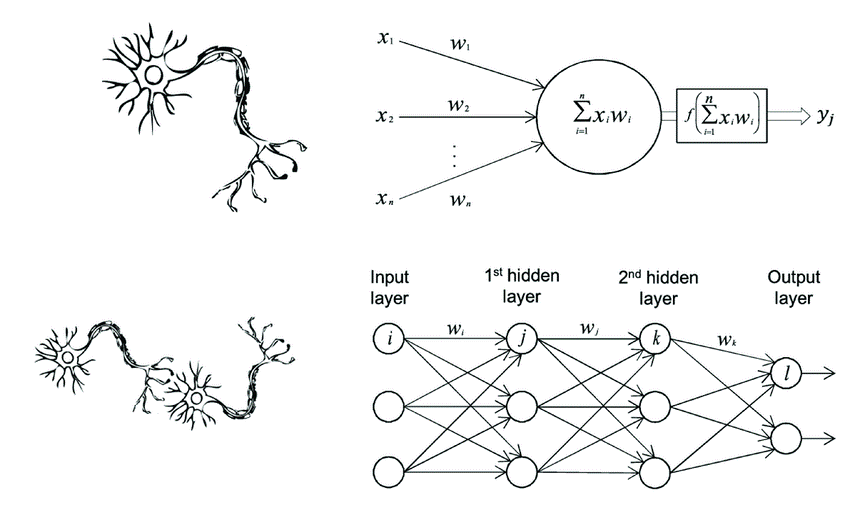
\includegraphics[width=1.0\linewidth]{Images/Chapter2/neuron}
\caption{مدلسازی یک نورون عصبی توسط رابطه ریاضی و ارتباط بین نرون‌ها با استفاده از لایه‌های پنهان
\cite{brainmentorsIntroductionDeep}}
\label{fig:ch2-neuron}
\end{figure}


\subsubsection{تابع خطا و پس‌انتشار
\protect\LTRfootnote{backpropagation}}
تابع خطا
 \LTRfootnote{Loss Function}
  نقش کلیدی در آموزش شبکه‌های عصبی دارد. این تابع تفاوت بین خروجی پیش‌بینی‌شده
  \lr{ \(y_{\text{pred}}\)}
   و خروجی واقعی
    \lr{\(y_{\text{true}}\)}
     را محاسبه می‌کند. یکی از رایج‌ترین توابع خطا، خطای 
  \lr{Binary Cross Entropy(BCE)}
   است که طبق 
   \autoref{eq:bce_loss}
   برای مسائل دسته‌بندی دوتایی استفاده می‌شود.

\begin{latin}
\begin{equation}
\label{eq:bce_loss}
L(\mathbf{y}_{\text{true}}, \mathbf{y}_{\text{pred}}) = -\frac{1}{m} \sum_{i=1}^{m} \left[ y_{\text{true}}^{(i)} \log(y_{\text{pred}}^{(i)}) + (1 - y_{\text{true}}^{(i)}) \log(1 - y_{\text{pred}}^{(i)}) \right]
\end{equation}
\end{latin}


هدف از آموزش شبکه، کمینه‌سازی این تابع خطا است که با استفاده از الگوریتم پس‌انتشار انجام می‌شود. در این روش، گرادیان
\LTRfootnote{Gradient}
 تابع خطا نسبت به هر وزن \(w_i\) طبق \autoref{eq:gradient} و قانون مشتقات زنجیره‌ای، محاسبه شده و سپس وزن‌ها با استفاده از قانون گرادیان کاهشی مطابق \autoref{eq:weight_update} به‌روزرسانی می‌شوند:

\begin{latin}
\begin{equation}
\label{eq:gradient}
\frac{\partial L}{\partial w_i}
\end{equation}
\end{latin}

\begin{latin}
\begin{equation}
\label{eq:weight_update}
w_{i+1} \leftarrow w_i - \eta \frac{\partial L}{\partial w_i}
\end{equation}
\end{latin}

\subsubsection{لایه‌های پرسپترون
\protect\LTRfootnote{Perceptron}
 چندلایه}
لایه‌های پرسپترون چندلایه
 \lr{(MLP)} 
 یکی از ساده‌ترین و پایه‌ای‌ترین ساختارها در شبکه‌های عصبی هستند. این لایه‌ها از تعدادی نورون تشکیل شده‌اند که به صورت کامل به یکدیگر متصل هستند؛ به بیان دیگر هر نورون در یک لایه به تمامی نورون‌های لایه‌ی قبلی متصل می‌شود و اطلاعات را به لایه‌ی بعدی منتقل می‌کند. خروجی هر لایه \(a^{[l]}\) از ترکیب خطی ورودی‌ها و اعمال تابع فعال‌سازی طبق \autoref{eq:mlp_output} به دست می‌آید:

\begin{latin}
\begin{equation}
\label{eq:mlp_output}
a^{[l]} = \phi(W^{[l]} a^{[l-1]} + b^{[l]})
\end{equation}
\end{latin}

\subsubsection{شبکه عصبی پیچشی
\protect\LTRfootnote{Convolutional Neural Network}}
برای بهبود عملکرد شبکه‌های عصبی در پردازش تصاویر، از لایه‌های شبکه عصبی پیچشی
\lr{(CNN)} 
استفاده می‌شود. در این لایه‌ها، عملیات کانولوشن به جای ضرب ماتریسی بین ورودی و وزن‌ها طبق \autoref{eq:convolution} انجام می‌شود. این عملیات برای هر ناحیه کوچک از تصویر با استفاده از یک فیلتر \(k\) صورت می‌گیرد.

\begin{latin}
\begin{equation}
\label{eq:convolution}
z_{i,j} = (X * k)_{i,j} = \sum_{m}\sum_{n} X_{i+m,j+n} \cdot k_{m,n}
\end{equation}
\end{latin}

خروجی این عملیات، نقشه ویژگی
\lr{Feature Map}
 است که به لایه بعدی منتقل می‌شود. با عبور یک تصویر از لایه‌های یک شبکه عصبی پیچشی، بین پیکسل‌های کنارهم در تصویر، یک رابطه برقرار می‌شود که درنتیجه آن، نقشه ویژگی استخراج شده برای هر پیکسل،‌ به وضعت پیکسل‌های اطرافش بستگی دارد و هرچه از پیکسل مبدا دور شویم، اثر آن در نقشه ویژگی کاهش پیدا می‌کند.
 
 




\subsubsection{بهینه‌سازها و الگوریتم 
\lr{Adam}
}

بهینه‌سازی یکی از مهم‌ترین اجزا در آموزش شبکه‌های عصبی هستند که هدف آنها به‌روزرسانی وزن‌ها به گونه‌ای است که تابع خطا به حداقل مقدار خود برسد. برای این منظور، از الگوریتم‌هایی استفاده می‌شود که بهینه‌ساز نامیده می‌شوند. 
یکی از رایج‌ترین بهینه‌سازها، الگوریتم گرادیان کاهشی است که در آن وزن‌ها در جهت منفی گرادیان تابع خطا به‌روزرسانی می‌شوند، هرابطه گرادیات کاهشی در \autoref{eq:weight_update} نشان داده شده است. 
 یکی دیگر از بهینه‌سازهای پیشرفته و کارآمد، بهینه‌ساز 
\lr{Adam}
 است. این بهینه‌ساز از ترکیب دو روش
\lr{Momentum}
 و
\lr{RMSProp}
 بهره می‌برد 
 \cite{towardsdatascienceUnderstandingDeep,mediumMomentumRMSpropAdam}.
  به‌روزرسانی وزن‌ها در \lr{Adam} با استفاده از روابط در 
  \autoref{eq:adam}
  انجام می‌شود.

\begin{latin}
\begin{equation}
\label{eq:adam}
\begin{aligned}
m_t &= \beta_1 m_{t-1} + (1 - \beta_1) \nabla L(\theta_t)\\
v_t &= \beta_2 v_{t-1} + (1 - \beta_2) (\nabla L(\theta_t))^2\\
\theta_{t+1} &= \theta_t - \eta \frac{\hat{m}_t}{\sqrt{\hat{v}_t} + \epsilon}
\end{aligned}
\end{equation}
\end{latin}


در این معادلات، \(m_t\) و \(v_t\) به ترتیب تخمین میانگین حرکت‌دار گرادیان و میانگین حرکت‌دار مربعات گرادیان در زمان \(t\) هستند، و \(\beta_1\) و \(\beta_2\) ضرایب مربوط به این میانگین‌ها هستند. \(\eta\) نرخ یادگیری و \(\epsilon\) یک مقدار بسیار کوچک برای جلوگیری از تقسیم بر صفر است. 
\lr{Adam} به دلیل توانایی خود در تنظیم نرخ یادگیری برای هر پارامتر به‌طور خودکار، به یکی از پرکاربردترین بهینه‌سازها در آموزش شبکه‌های عصبی عمیق تبدیل شده است. 


\section{مدل‌های طبقه‌بندی در شبکه عصبی عمیق}

\subsection{\lr{ResNet}}
\label{ResNet subsection}
شبکه‌های عصبی عمیق به یک ابزار قدرتمند در انجام وظایف مختلف یادگیری ماشین تبدیل شده‌اند. با این حال، با افزایش عمق این شبکه‌ها، مشکلاتی همچون ناپدیدشدن مشتق
\LTRfootnote{Vanishing Gradient}
یا انقجار مشتق 
\LTRfootnote{Exploding Gradient}
 و دشوار شدن آموزش به‌وجود می‌آید. برای حل این مشکلات،
  \lr{He}\cite{he2016deep}
   و همکارانش معماری شبکه‌های 
   \lr{ResNet}
   را پیشنهاد کردند که امکان آموزش شبکه‌های بسیار عمیق‌تر را با معرفی اتصالات 
   \lr{Residual}
   فراهم می‌کند.
ایده اصلی پشت 
\lr{ResNet}
 معرفی یک اتصال میانبر
 \LTRfootnote{Skip Connection}
 است که یک یا چند لایه از شبکه را دور می‌زند. این اتصال میانبر به شبکه امکان می‌دهد تا از طریق آن، مشتق خطا به لایه‌های ابتدایی برسد تا فرایند آموزش برای لایه‌هایی که از خروجی دور هستند، با مشکل مواجه نشود.همانطور که در 
 \autoref{fig:ch-2resnet_block}
 نمایش داده‌‌شده است، در شبکه‌های 
 \lr{ResNet}
 به جای یادگیری یک نگاشت مستقیم، مثلاً $H(x)$، شبکه نگاشت $F(x) = H(x) - x$ را یاد می‌گیرد که بهینه‌سازی آن ساده‌تر است. بنابراین، خروجی نهایی بلوک
 \LTRfootnote{Block}
  $H(x) = F(x) + x$ خواهد بود که در نتیجه آن، مشتق
 تابع خطای $L$ به‌ازای ورودی $x$ در 
 \autoref{eq:ch2-resnet-deriviation}
 نمایش‌ داده‌شده است.
 
\begin{latin}
\begin{equation}
\label{eq:ch2-resnet-deriviation}
\begin{aligned}
 \frac{\partial L}{\partial x} = \frac{\partial L}{\partial H(x)} \cdot \frac{\partial H(x)}{\partial x} = \frac{\partial L}{\partial H(x)} \cdot \left(1 + \frac{\partial F(x)}{\partial x}\right)
\end{aligned}
\end{equation}
\end{latin}

 
 این فرمول نشان می‌دهد که مشتق می‌تواند به راحتی از طریق مسیر میانبر عبور کند، که به حل مشکل ناپدید شدن یا انفجار گرادیان کمک می‌کند.
 
\begin{figure}[h]
    \centering
    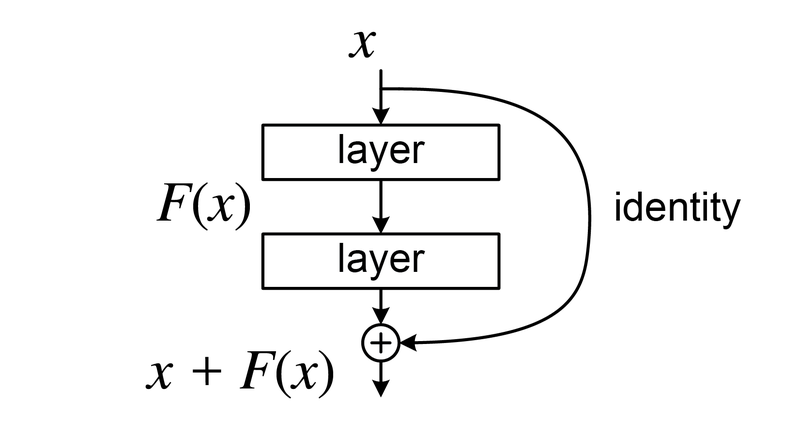
\includegraphics[width=0.6\textwidth]{Images/Chapter2/ResBlock.png}
    \caption{یک بلوک از معماری 
    \lr{ResNet} 
    که اتصال میانبر همانی را نشان می‌دهد
    \cite{wikipediaResidualNeural}.}
    \label{fig:ch-2resnet_block}
\end{figure}
\lr{ResNet}
 در انجام وظیفه طبقه‌بندی تصویر، عملکرد مناسبی از خود نشان‌داده است. این شبکه با معرفی اتصال میانبر و  فراهم کردن امکان آموزش شبکه‌های بسیار عمیق، باعث بهبود عملکرد مدل‌های شبکه عصبی عمیق شده‌ است.


\subsection{\lr{ResNeXt}}

\lr{ResNeXt}
توسط 
\lr{Xie}\cite{xie2017aggregated}
و همکاران معرفی شده است که 
یک معماری شبکه عصبی پیچشی عمیق است که براساس ساختار 
\lr{ResNet}
ساخته شده و با معرفی یک فراپارامتر
\LTRfootnote{Hyper-parameter}
 جدید به نام کاردینالیتی
\LTRfootnote{Cardinality} 
  سعی در بهبود مدل 
  \lr{ResNet}
  داشته‌است.
 این مدل به منظور بهبود عملکرد شبکه‌های عصبی عمیق،  مسیرهای موازی متعدد را در ساختار شبکه ایجاد می‌کند که این روش مشابه مدل ساختار
  \lr{Inception} 
می‌باشد اما با تفاوت‌های کلیدی در سادگی طراحی اجزای شبکه.

همانطور که در 
\autoref{fig:ch2-resnext1}, \autoref{fig:ch2-resnext2}
مشخص شده است، مسیرهای موازی در ساخار شبکه ایجاد شده است که این مسیرها به مقدار کاردینالیتی بستگی دارد.
کاردینالیتی به تعداد مسیرهای موازی درون هر بلوک شبکه اشاره دارد. برخلاف افزایش عمق یا عرض که به افزایش تعداد لایه‌ها یا پیچیدگی هر لایه منجر می‌شود، افزایش کاردینالیتی اجازه می‌دهد که چندین مسیر پردازشی به صورت موازی عمل کنند و در نهایت خروجی‌های آن‌ها با یکدیگر ادغام شوند که از بار پردازشی شبکه کم می‌کند.
\autoref{fig:ch2-resnext3}
ساده‌سازی بلوک 
\lr{ResNeXt}
برای بهینه‌سازی و ساده‌سازی محاسبات را نشان می‌دهد که از لایه‌های پیچشی گروهی استفاده می‌کند. در این روش، کانال‌های 
\LTRfootnote{Channel}
ورودی به گروه‌های مختلف تقسیم می‌شوند و کانولوشن‌ها به صورت مستقل در هر گروه انجام می‌گیرند.
افزایش کاردینالیتی در \lr{ResNeXt} نه تنها باعث بهبود دقت مدل می‌شود، بلکه امکان استفاده از مسیرهای پردازشی متعدد به صورت موازی، بدون افزایش چشمگیر در پیچیدگی محاسباتی، را فراهم می‌کند. این ویژگی به \lr{ResNeXt} اجازه می‌دهد که در وظایف پیچیده مانند طبقه‌بندی تصاویر با دقت بیشتری عمل کند. علاوه بر این، استفاده از لایه‌های پیچشی گروهی به کاهش هزینه محاسباتی کمک کرده و در عین حال، قدرت الگوهای پیچیده را حفظ می‌کند.

\begin{figure}[h!]
    \centering % <-- added
    \begin{subfigure}{0.33\textwidth}
        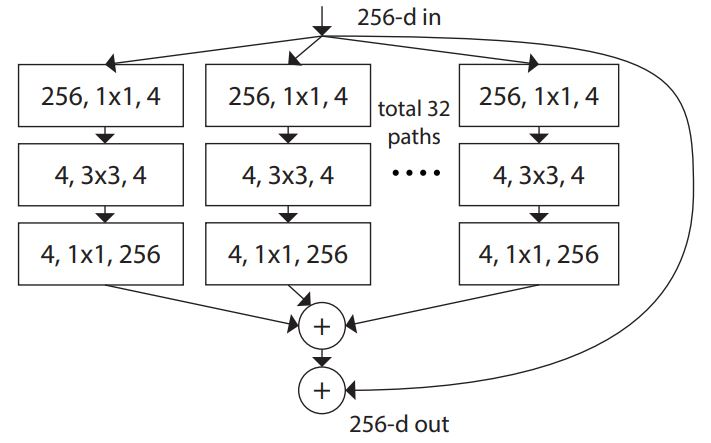
\includegraphics[width=\linewidth]{Images/Chapter2/resnext1.JPG}
        \caption{}
        \label{fig:ch2-resnext1}
    \end{subfigure}\hfil % <-- 
    \begin{subfigure}{0.33\textwidth}
        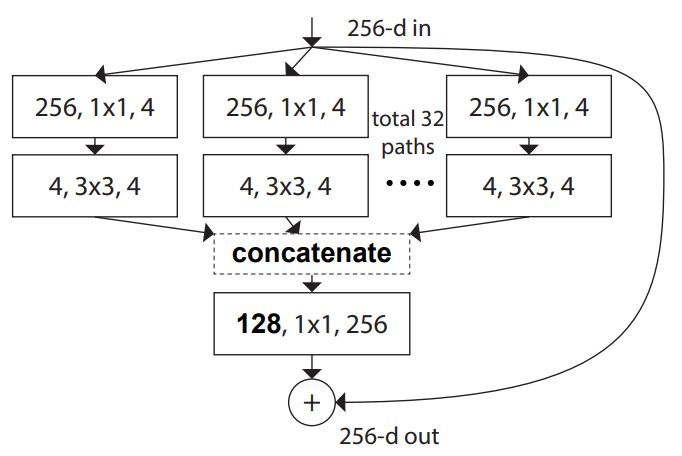
\includegraphics[width=\linewidth]{Images/Chapter2/resnext2.JPG}
        \caption{}
        \label{fig:ch2-resnext2}
    \end{subfigure}\hfil % <-- added
    \begin{subfigure}{0.33\textwidth}
        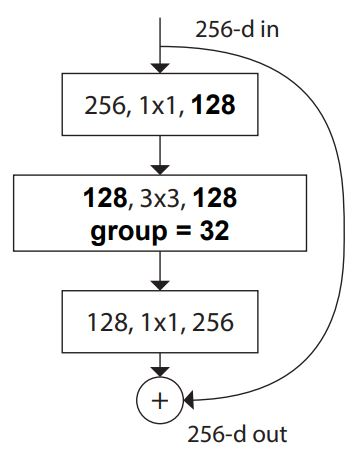
\includegraphics[width=\linewidth]{Images/Chapter2/resnext3.JPG}
        \caption{}
        \label{fig:ch2-resnext3}
    \end{subfigure}
    \caption{ساختارهای مختلف در معماری 
    \lr{ResNeXt}
     که کانولوشن‌های گروهی، مسیرهای پردازشی موازی و روش ادغام را نشان می‌دهند
     \cite{xie2017aggregated}.}
    \label{fig:fig:ch2-resnext}
\end{figure}







\subsection{شبکه
\lr{Squeeze-and-Excitation}
\lr{(SENet)}}

\lr{Hu}\cite{hu2018squeeze}
و همکاران،‌ با معرفی بلوک
 \lr{Squeeze-and-Excitation}
 \lr{(SE)}
 ، دقت طبقه‌بندی در \lr{ImageNet} به میزان 2.5\% نسبت به سال گذشته بهبود یافت. این بلوک با وزن‌دهی به میان کانال‌های مختلف در هر لایه از شبکه‌عصبی پیچشی، عملکرد شبکه‌های عصبی را با هزینه محاسباتی بسیار کمی بهبود می‌بخشد.
ایده اصلی درمورد روش 
 \lr{Squeeze-and-Excitation}
  این است که در یک لایه معمولی در شبکه عصبی پیچشی، ارزش هر کانال در ورودی شبکه، با بقیه کانال‌ها یکسان است. بلوک \lr{SE} اما، رویکردی تطبیقی را معرفی می‌کند که در آن اهمیت هر کانال به طور جداگانه و بر اساس زمینه ارزیابی می‌شود و به آن وزنی خاص اختصاص‌داده می‌شود.

\autoref{fig:se_block}
نحوه عملکرد این مدل را نشان می‌دهد که در گام نخست از هر کانال نقضه ویژگی میانگین گرفته می‌شود، سپس این میانگین از یک تابع خطی عبور داده می‌شود و در گام بعدی، تابع 
\lr{Sigmoid}
روی آن اعمال می‌شود تا وزن‌ها بین 0 تا 1 قرار بگیرند.
در انتها وزن‌های محاسبه شده در نقشه ویژگی ضرب می‌شود و خروجی لایه پیچشی 
 \lr{Squeeze-and-Excitation}
 شبکه عصبی پیچشی به‌دست می‌آید.
 \lr{ResNeXt}
 یکی از مدل‌های پایه‌ای است که با استفاده از روش بلوک
 \lr{SE}
 عملکردش ارتقا پیدا کرده است.
 
\begin{figure}[h!]
    \centering
    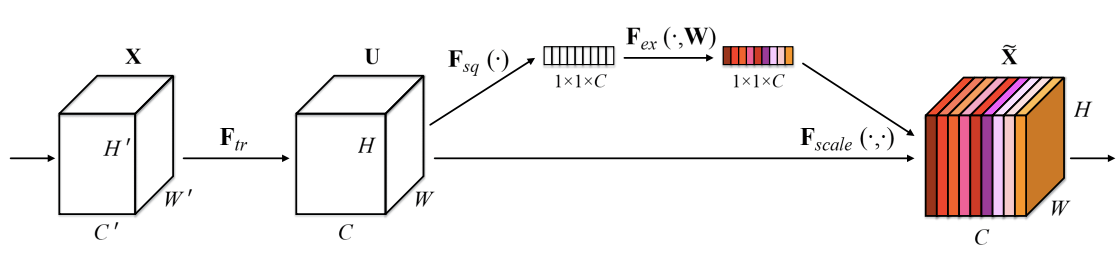
\includegraphics[width=1\textwidth]{Images/Chapter2/squeeze and excitation.png}
    \caption{بلوک \lr{Squeeze-and-Excitation} که نحوه عملکرد آن را در ارزیابی و وزن‌دهی کانال‌ها نشان می‌دهد \cite{hu2018squeeze}.}
    \label{fig:se_block}
\end{figure}




\subsection{\lr{DenseNet}}

\lr{DenseNet}
یک نوع شبکه‌ عصبی پیچشی است که به‌منظور بهبود عملکرد شبکه‌های عصبی پیچشی سنتی معرفی شده‌است. هدف اصلی این شبکه، کاهش محدودیت‌هایی است که معمولاً شبکه‌های پیچشی عمیق، با آن‌ها مواجه می‌شوند.
در شبکه‌های پیچشی سنتی، یکی از مشکلات اصلی زمانی رخ می‌دهد که مشتق، نمی‌تواند در فرایند پس‌انتشار به درستی در تمامی لایه‌ها انتقال یابد که این مسئله در
\autoref{ResNet subsection}
بررسی شده است. مسئله ناپدید شدن مشتق به ویژه در لایه‌های اولیه بسیار تاثیر می‌گذارد که این موضوع به‌روزرسانی وزن‌ها و بایاس‌ها را مختل کرده و بر عملکرد کلی شبکه تأثیر منفی می‌گذارد.
برای کمک به کاهش مشکلاتی که پیشتر مطرح شد
\cite{huang2017densely}.
\lr{Huang}\cite{huang2017densely}
و همکاران، مدل 
 \lr{DenseNet}
 ‌را معرفی کردند. در حالی که یک بلوک‌های شبکه عصبی پیچشی‌ سنتی، تنها از نقشه ویژگی خروجی فعلی به عنوان ورودی برای لایه بعدی استفاده می‌کنند،
  \lr{DenseNet}
   علاوه بر آن، تمامی نقشه‌های ویژگی که در لایه‌های پیشین ایجاد شده را نیز در ورودی لایه فعلی استفاده می‌کند. همانطور که در \autoref{fig:densenet_architecture} مشاهده می‌شود. این کار جریان اطلاعات بین لایه‌ها را به حداکثر می‌رساند، تعداد متغییرهای مدل را افزایش چشمگیری نمی‌دهد و به طور قابل توجهی مشکل ناپدید شدن گرادیان‌ها را بهبود می‌بخشد .

شبکه‌های 
\lr{DenseNet}،
 برخلاف
  \lr{ResNet}
  ‌ها که از جمع برای ترکیب نقشه‌های ویژگی استفاده می‌کنند، از الحاق 
  \LTRfootnote{Concatenation}
   استفاده می‌کنند تا اطلاعات را به صورت موثرتری حفظ کنند. هر لایه در
    \lr{DenseNet} 
    نقشه‌های ویژگی تمامی لایه‌های قبلی را به عنوان ورودی دریافت کرده و آن‌ها را قبل از عبور از تبدیل غیرخطی به یکدیگر الحاق می‌کند \cite{huang2017densely}.

\begin{figure}[h]
    \centering
    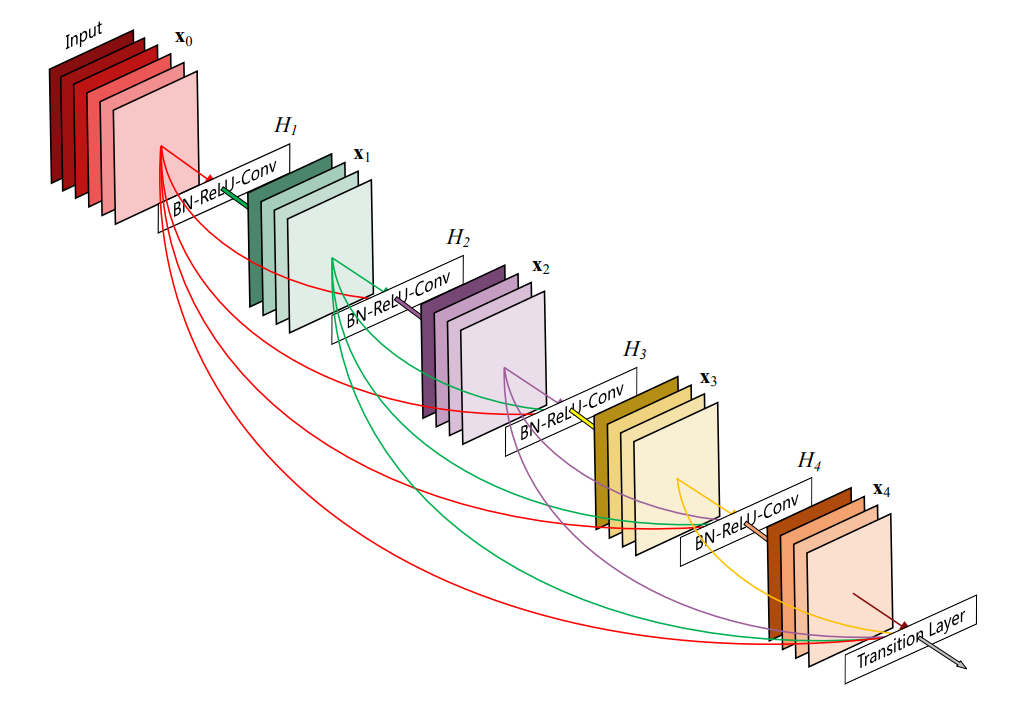
\includegraphics[width=1\textwidth]{Images/Chapter2/DenseNet.PNG}
    \caption{معماری یک بلوک
     \lr{DenseNet}\cite{huang2017densely}.}
    \label{fig:densenet_architecture}
\end{figure}






\subsection{\lr{EfficientNet}}

\lr{Tan}\cite{tan2019efficientnet} 
 و همکارانش یک معماری و روش مقیاس‌گذاری را در مدلی به نام 
 \lr{EfficientNet}
  معرفی کردند. این روش به ما امکان می‌دهد که تعداد متغیرهای مدل را به صورت بهینه افزایش دهیم. در این روش، برای افزایش تعداد متغیرهای مدل، سه ویژگی عمق، عرض و وضوح
   \LTRfootnote{Resolution}
  تصویر باید به صورت یکنواخت و با استفاده از سه ضریب ثابت افزایش پیدا کنند.

به طور مشخص، اگر بخواهیم تعداد متغییر‌های مدل را به میزان \(2^N\) برابر افزایش دهیم، می‌توانیم به سادگی عمق شبکه را به میزان \( \alpha^N \)، عرض شبکه را به میزان \( \beta^N \) و وضوح تصویر را به میزان \( \gamma^N \) افزایش دهیم، که در آن \(\alpha\)، \(\beta\) و \(\gamma\) ضرایب ثابتی هستند که 
\autoref{eq:ch2-EffNet}
باید برای آنها برقرار باشد. این رابطه به این معناست که افزایش منابع محاسباتی به میزان \(2^N\) برابر، به توزیع متناسبی از افزایش عمق، عرض و وضوح تصویر منجر می‌شود. 

 
\begin{latin}
\begin{equation}
\label{eq:ch2-EffNet}
\begin{aligned}
\alpha \times \beta^2 \times \gamma^2 \approx 2
\end{aligned}
\end{equation}
\end{latin}

 در نتیجه پژوهش 
 \lr{Tan}
  و همکارانش، یک خانواده از مدل‌های مبتنی بر شبکه عصبی پیچشی ایجاد شد که ضمن داشتن تعداد متغییرهای بسیار کمتر، عملکرد بهتری نسبت به مدل‌های قبلی ایفا می‌کند.
 

\section{مدل‌های قطعه‌بندی در شبکه عصبی عمیق}

\subsection{\lr{U-Net}}

شبکه
 \lr{U-Net} 
 یکی از پرکاربردترین معماری‌ها در حوزه‌ی پردازش تصویر و به‌ویژه در بخش‌بندی تصاویر است که توسط
 \lr{Ronneberger}\cite{ronneberger2015u}
 و همکاران توسعه داده‌شده است. این مدل، که در اصل به‌عنوان یک شبکه عصبی پیچشی خودرمزگذار
  \LTRfootnote{Autoencoder}
   معرفی شد، به دلیل طراحی خاص خود که امکان بازیابی دقیق اطلاعات مکانی را به کمک مسیرهای میانبر فراهم می‌آورد، به‌طور گسترده‌ای مورد استفاده قرار می‌گیرد.

ساختار \lr{U-Net} شامل دو مسیر اصلی است؛ 
مسیر اول، رمزگذار نام دادرد که مسئول استخراج ویژگی‌ها و کاهش ابعاد و افزایش تعداد کانال‌ها است.
مسیر بعدی،‌رمزگشا نام دارد که وظیفه بازسازی تصویر به اندازه اصلی و مشخص کردن محل جسم را برعهده دارد که این کار را با استفاده از اطلاعات استخراج‌شده از مسیر رمزگذار انجام می‌دهد.

ساختار شبکه 
 \lr{U-Net} 
در \autoref{fig:unet_architecture} مشاهده می‌شود که مسیر رمزگذار شامل چندین مرحله از شبکه عصبی پیچشی و لایه ادغام
 \LTRfootnote{Pooling}
 است. از سوی دیگر، مسیر رمزگشا شامل افزایش ابعاد و ترکیب ویژگی‌های استخراج‌شده در مسیر رمزگذار است تا تصویر نهایی با دقت بالایی بازسازی شود. یکی از ویژگی‌های کلیدی
  \lr{U-Net}
  مسیرهای میانبر بین لایه‌های رمزگذار و رمزگشا متناظر است که اطلاعات مکانی دقیق را از رمزگذار به رمزگشا منتقل می‌کند.

\begin{figure}[h]
    \centering
    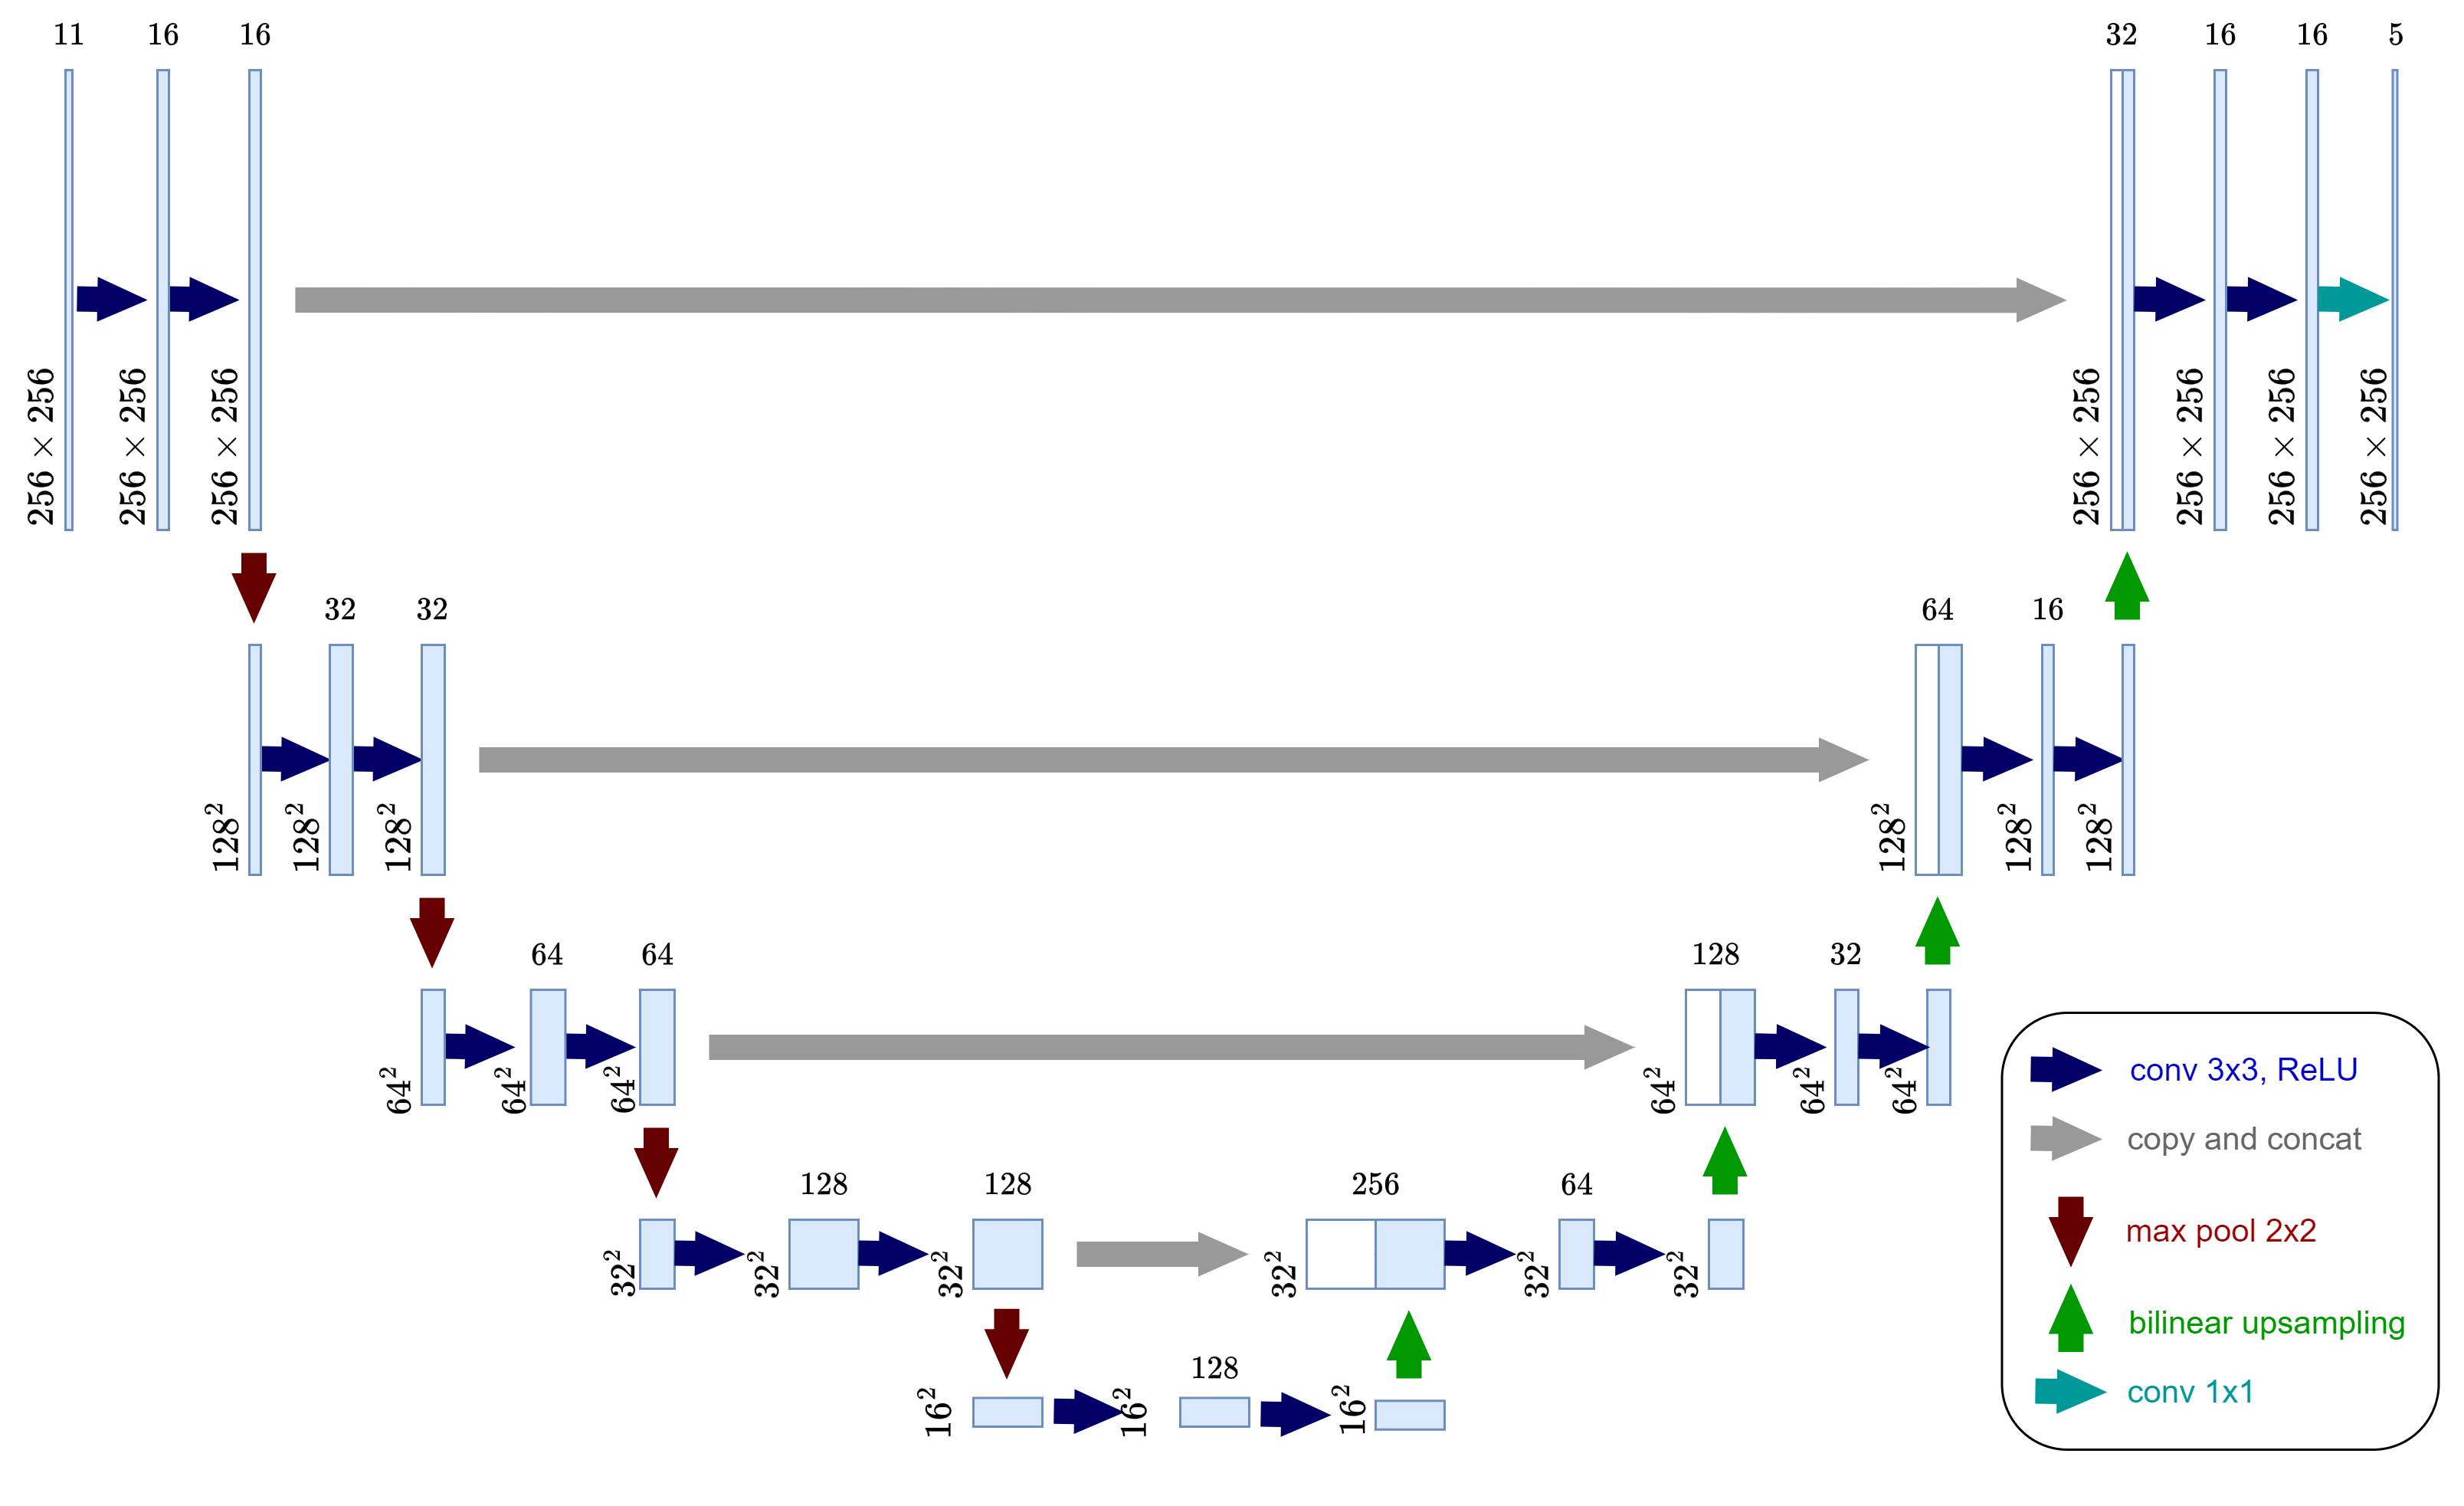
\includegraphics[width=1\textwidth]{Images/Chapter2/U-Net.drawio.png}
    \caption{ساختار شبکه \lr{U-Net} که شامل مسیر رمزگذار و رمزگشا، همراه با اتصالات کپی و الحاق است
    \cite{ronneberger2015u}.}
    \label{fig:unet_architecture}
\end{figure}

در حالی که ساختار اصلی \lr{U-Net} به‌خوبی قادر به انجام وظایف مختلف است، امکان بهبود عملکرد آن با استفاده از مدل‌های پیشرفته‌تر در بخش رمزگذار وجود دارد. به عنوان مثال، می‌توان از مدل‌هایی که در بخش‌های قبل مطرح شد،‌ مانند
 \lr{ResNet}، \lr{ResNeXt}، \lr{SENet} و \lr{EfficientNet}
  در مسیر رمزگذار
   \lr{U-Net} 
   استفاده کرد. این مدل‌ها به دلیل قابلیت‌های قدرتمند خود در استخراج ویژگی‌ها و مدیریت اطلاعات پیچیده، می‌توانند عملکرد
    \lr{U-Net} 
    را در وظایف پیچیده‌تر به‌طور قابل توجهی بهبود بخشند. 
این قابلیت به‌ویژه در مواقعی که تصاویر ورودی دارای جزئیات بسیار بالایی هستند یا نیاز به دقت بالایی در خروجی است، اهمیت بیشتری پیدا می‌کند. به همین دلیل، \lr{U-Net} با ساختار خود، یکی از انعطاف‌پذیرترین مدل‌ها برای ترکیب با معماری‌های دیگر به‌شمار می‌رود و به‌طور گسترده در زمینه‌های مختلف از جمله پزشکی و بینایی ماشین مورد استفاده قرار می‌گیرد.





\section{پس‌پردازش}
\label{ch2-post-process}
پس‌پردازش پیشنهادی در این پژوهش، به منظور بهبود عملکرد مدل قطعه‌بندی، توسعه داده شده است.
\autoref{fig:ct2-3d}
یک نمونه تصویر سی‌تی‌اسکن را نشان می‌دهد؛ همانطور که در این تصویر مشخص است،‌ حاشیه سیاه برش‌ها شامل هیچ اندامی نمی‌باشد و بدیهی است که هیچ ضایعه خونریزی در این نواحی یافت نخواهد شد، بنابراین با توجه‌به اینکه یکای 
 \lr{Hounsfield}
 این نواحی بسیار از مقدار آن در بافت مغز متفاوت است، روش آستانه‌گذاری روی برش‌ها اعمال شد که آستانه مربوطه از روی 
\autoref{fig: ch2-slice hist lim}،
به گونه‌ای انتخاب شد که نواحی شامل بافت مغز،‌از نواحی که هیچ اندامی در آنها وجود ندارد جدا شود.
\autoref{fig:ch2-post-process-mask}
لایه‌های پس‌پردازش استخراج‌شده با روش آستانه‌گذاری را برای برش‌های متفاوت نشان می‌دهد. این لایه‌ها پس از آنکه استخراج شدند،‌ در مرحله تصمیم‌گیری مدل قطعه‌بندی مورد استفاده قرار گرفته می‌شوند. روش استفاده از این لایه‌ها به گونه‌ای است که احتما هرگونه پیش‌بینی موجود در نواحی سیاه از تصویر را برابر 0 قرار می‌دهد و باعث می‌شود تا نیاز به آموزش لایه‌های مدل قطعه‌بندی  در این نواحی لازم نباشد.




\begin{figure}[h]
\centering
\includegraphics[width=1.0\linewidth]{"Images/Chapter2/post-process mask"}
\caption{نمونه لایه‌های پس‌پردازش استخراج شده از برش‌های بیمار}
\label{fig:ch2-post-process-mask}
\end{figure}




\section{روش پیشنهادی}
هدف اصلی در این پژوهش،‌ بهبود عملکرد مدل‌های قطعه‌بندی در تصاویر سی‌تی‌اسکن بوده به گونه‌ای که این روش به صورت عام، امکان پیاده‌سازی روی مدل‌های قطعه‌بندی را داشته باشد. به منظور توسعه این روش،‌ ناترازی داده‌ها،‌ به عنوان یکی از اصلی‌ترین مشکلات در پردازش تصاویر سه‌بعدی پزشکی و سی‌تی‌اسکن مورد مطالعه قرار گرفت.

ناترازی در داده‌های سی‌تی‌اسکن، خصوصا برای پردازش خونریزی درون‌جمجمه‌ای، می‌تواند در سه سطح بیمار‌محور، برش‌محور و پیکسل‌محور رخ دهد که در مجموعه‌داده موجود،‌ این ناترازی تنها در دو سطح برش‌محور و پیکسل‌محور رخ داده است. 
\autoref{fig: ch2-patient distrbiution}
پراکندگی داده را به‌صورت بیمارمحور و 
\autoref{fig: ch2-slice distribution}
پراکندگی داده را به‌صورت برش‌محور نشان می‌دهد که ناترازی در سطح برش، بسیار شدید می‌باشد. 
پراکندگی پیکسل‌های دارای خونریزی نیز در این مجموعه‌داده، به گونه‌ای است که در برش‌هایی که ضایعه خونریزی وجود دارد، تعداد پیکسل‌های دارای خونریزی، در حدود 2000 پیکسل می‌باشد که این مقدار در برابر تعداد پیکسل‌های کل برش که برابر 
$2^{18}$
پیکسل می‌باشد،‌ نشان‌دهنده شدت بیشتر ناترازی در سطح پیکسل می‌باشد.

برای کاهش مشکل ناترازی در سطح برش، یک روش دو مرحله‌ای، توسعه داده‌شد که به موجب آن،‌ در گام نخست برش‌های سی‌تی‌اسکن طبقه‌بندی خواهند شد تا وجود ضایعه تشخیص داده‌شود و در گام بعدی،‌ برش‌هایی که دارای بیماری پیش‌بینی شده‌اند،‌ به یک شبکه قطعه‌بندی ارسال می‌شوند تا مراحل قطعه‌بندی در این برش‌ها طی شود.
استفاده از این روش برای پردازش تصاویر سی‌تی‌اسکن،‌این مزیت را دارد که با حذف برش‌های سالم از فرایند تصمیم‌گیری، باعث کاهش تعداد پیکسل‌هایی می‌شود که به صورت اشتباه،‌ به عنوان پیشکسل‌های دارای ضایعه خونریزی درنظر گرفته شده‌اند. نکته حائز اهمیت درمورد این روش این است که تمام خطاهایی که در مدل طبقه‌بندی رخ بدهند، مستقیما در عملکرد مدل قطعه‌بندی تاثیر می‌گذارند خصوصا اگر برشی که دارای خونریزی بوده، به عنوان برش سالم درنظر گرفته شود بنابراین باید توجه داشت تا آستانه تصمیم‌گیری در این روش به گونه‌ای انتخاب شود تا تعداد برش‌هایی که واقعا سالم نیستند اما سالم تشخیص‌داده می‌شوند به حداقل مقدار خود برسد. حد بالای پیشنهادی برای این آستانه به گونه‌ای است که به موجب آن، تمام سی‌تی‌اسکن‌های دارای خونریزی  موجود در مجموعه‌داده به درستی تشخیص داده‌شوند (تشخیص بیمار‌محور). 

استفاده از روش پس‌پردازش مذکور در 
\autoref{ch2-post-process}،
باعث می‌شود تا ناترازی در سطح پیکسل تا حد خوبی کاهش پیدا کند و ب موجب آن فرایند آموزش مدل، بیشتر معطوف به شناسایی نواحی دارای خونریزی شود تا اینکه یک قسمت از فرایند آموزش مدل صرف این شود تا نواحی خارج از جمجمه شناسایی شود. این پس‌پردازش به ما این امکان را می‌دهد تا با کاهش میزان آستانه تصمیم، تعداد پیکسل‌هایی که به درصتی درون جمجمه شناسایی می‌شوند را افزایش دهیم. پس‌پردازش مذکور در پژوهش، به‌صورت مجتمع در فرایند آموزش استفاده شده است.
\begin{figure}[h]
\centering
\includegraphics[height=0.5\textheight]{"Images/Chapter2/block diagram of 2 step .drawio"}
\caption{روندنمای روش پیشنهادی در این پژوهش}
\label{fig:ch2-block-diagram-of-2-step}
\end{figure}

\autoref{fig:ch2-block-diagram-of-2-step}
روندنمای روش پیشنهادی و پس‌پردازش را به منظور بررسی برش‌های خونریزی نشان می‌دهد که در این پردازش استفاده شده‌است. همانطور که از این روند‌نما مشخص است، این روند بستگی به مدل طبقه‌بندی و قطعه‌بندی مورد استفاده ندارد و می‌توان از هر مدلی در این روند استفاده کرد که این مسئله باعث افزایش قابلیت توسعه و نگهداری نرم‌افزارهایی می‌شود که بر پایه این روند توسعه داده‌ شده‌اند.

\section{آموزش و تصمیم‌گیری}

\subsection{طبقه‌بندی}

گام نخست در این پژوهش، آموزش یک مدل طبقه‌بندی مناسب به منظور استفاده در روش دو مرحله‌ای است که به‌موجب آن یک جستجوی شبکه‌ای 
\LTRfootnote{Grid Search}
با استفاده از مدل 
\lr{ResNet 50}
انجام شد. در این جستجوی شبکه‌ای،‌ با توجه به چالش‌ ناترازی مجموعه‌داده، از تابع هزینه 
\lr{Cross Entropy}
وزن‌دار استفاده شد و همچنین با استفاده از روش افزایش مصنوعی داده، جاگذاری داده
\LTRfootnote{Bootstrap}
و کاهش داده غالب در ضرایب متفاوت استفاده شد تا بهترین نتیجه ممکن برای مدل طبقه‌بندی یافت شود. 
\autoref{table:ch2-grid-values}
نمایش‌دهنده مقادیر مورد استفاده در جستجوی شبکه‌ای می‌باشد. در این جستجوی شبکه‌ای، کاهش داده غالب با توجه‌به توزیع برش‌های دارای خونریزی که در 
\autoref{fig:ch2-slice-hist}
نمایش داده شده است انجام شده تا داده‌هایی که کمترین تاثیر را در آموزش دارند،‌ با احتمال بیشتری کنار گذاشته شوند و ضریبی که در جدول 
\autoref{table:ch2-grid-values}
برای این روش اعلام شده،‌ به این معنی می‌باشد که نسبت برش‌های بیمار به برش‌های سالم پس از اعمال این روش، برابر ضریب اعلامی خواهد شد.
در ادامه افزایش مصنوعی داده و جایگذاری داده نیز‌ تنها به روی برش‌هایی با تشخیص خونریزی درون‌جمجمه‌ای صورت پذیرفته و تا متناسب  با پراکندگی برش‌های دارای خونریزی، افزایش این داده‌ها صورت پذیرد که در 
\autoref{fig:ch2-slice-hist}
توزیع این داده‌ها نمایش داده شده است و پس از اعمال این روش‌ها، تعداد برش‌های بیمار در ضریب اعلام شده ضرب شده است. باید توجه داشت که در جستجوی شبکه‌ای ابتدا  افزایش مصنوعی داده و جایگذاری داده اعمال شده و پس از آن کاهش داده غالب روی مجموعه‌داده اعمال شده است.
در آموزش مدل طبقه‌بندی، به علت وجود تعداد کم داده‌های دارای خونریزی و احتمال بیش‌برازش\LTRfootnote{Overfit}،
از روش 
\lr{5-fold-cross-validation}
استفاده شد. در گام نخست از استفاده از این روش، یک زیرمجموعه ارزیابی
\LTRfootnote{Test}
که 20 درصد از کل مجموعه‌داده می‌باشد، انتخاب شده‌است و پس از آن روی باقی مجموعه‌داده عملیات
\lr{5-fold-cross-validation}
را برای آموزش مدل انجام شده است؛ در انتها پس از فرایند آموزش، تنظیم متغییرهای تصمیم‌گیری‌ مدل‌های بدست‌آمده روی مجموعه‌داده ارزیابی انجام شده و سازوکار تصمیم‌گیری شورایی
\LTRfootnote{Voting}
نهایی شده است که این سازوکار در 
\autoref{ch2-decision-policy}
توضیح داده شده است.
در انتها مدل پیشنهادی روی مجموعه داده ارزیابی آزمایش شده است. استفاده از این روش باعث می‌شود تا از عملکرد مدل و مقاوم بودن آن اطمینان حاصل شود. به منظور اطمینان از اینکه متغییرهای بدست آمده در عملات جستجوی شبکه‌ای،‌ در بهبود عملکرد مدل‌های شبکه عصبی تاثیرگذار است، مدل‌های 
\lr{VGG16}،\lr{MobileNet-V2} و \lr{Inception‌-V3}
نیز با بهترین تنظیمات بدست آمده روی 
\lr{ResNet50} 
آموزش داده شد.

\begin{table}[h]
\centering
\caption{ضرایب مورد استفاده در جستجوی شبکه‌ای}
\label{table:ch2-grid-values}
\resizebox{\textwidth}{!}{%
\begin{tabular}{llll}
\textbf{روش}                       & \textbf{ضریب اول} & \textbf{ضریب دوم} & \textbf{ضریب سوم} \\ \hline
افزایش مصنوعی داده                 & $2$               & $2.5$             & $3.3$             \\
جایگذاری داده                      & $2$               & $2.5$             & $3.3$             \\
کاهش داده غالب                     & $1$               & $2$               & $3$               \\
افزایش وزن داده مثبت در تابع هزینه & $2$               & $4$               & $6$               \\
کاهش وزن داده منفی در تابع هزینه   & $0.5$             & $0.25$            & $-$               
\end{tabular}%
}
\end{table}

\subsection{قطعه‌بندی}
در این پژوهش،‌ مدل شبکه عصبی عمیق 
\lr{U-Net}
به عنوان ساختار اصلی برای آموزش وظیفه قطعه‌بندی درنظر گرفته شده است. به منظور آموزش این مدل یک جستجوی شبکه‌ای جامع روی مجموعه‌داده انجام شد. متناسب با نتایجی که به روی وظیفه طبقه‌بندی بدست آمده، استفاده از روش‌هایی مثل کاهش داده غالب و جایگذاری داده تاثیر مناسبی روی نتایج نداشته است بنابراین این دو روش در جستجوی شبکه‌ای مدل قطعه‌بندی استفاده نشده است. در آموزش مدل قطعه‌بندی به روش جسجتوی شبکه‌ای، از روش افزایش مصنوعی داده با ضرایب 
$3$، $4$، $5$ و $6$
به همراه انواع مختلف توابع هزینه شامل 
\lr{Dice}، \lr{Tversky}، \lr{Focal Tversky}، \lr{Focal}،  \lr{Cross-entropy} و
\lr{Cross-entropy}
وزن‌دار با وزن‌های 10، 100،‌ 200، 500 و 1000 برای پیکسل‌های مثبت و انواع مختلف رمزگذار در ساختار شبکه 
\lr{U-Net}
با ابعاد متفاوت شامل 
\lr{ResNet}، \lr{ResNeXt}، \lr{SE-ResNeXt}, \lr{EfficientNet}
و 
\lr{DenseNet}
استفاده شده است.

در مراحل آموزش مدل قطعه‌بندی، داده ارزیابی ابتدا از مدل شورایی طبقه‌بندی عبور داده شد و تمام برش‌هایی که در این مدل دارای خونریزی درون‌جمجمه‌ای تشخیص داده شده‌اند،‌ طبق روندنمای 
\autoref{fig:ch2-block-diagram-of-2-step}
به مدل قطعه‌بندی ارسال شدند تا برش‌ها قطعه‌بندی شوند.
درگام آخر، یک سازوکار تصمیم‌گیری شورایی که در 
\autoref{ch2-decision-policy}
توضیح داده شده است، 
برای قطعه‌بندی برش‌ها استفاده شد تا پیش‌بینی مدل‌های متفاوت مورد استفاده قرار گیرد.



\subsection{سازوکار تصمیم‌گیری شورایی}
\label{ch2-decision-policy}
استفاده از روش
\lr{5-fold-cross-validation}
برای ارزیابی مدل‌های شبکه‌ عصبی،‌ می‌تواند با یک سازوکار شورایی در لایه تصمیم‌گیری همراه شود که به موجب آن اثر بیش‌برازش روی مجموعه‌داده کاهش پیدا می‌کند. در این پژوهش،‌ یک روش شورایی ساده برای وظیفه طبقه‌بندی پیشنهاد شده است که به‌موجب آن، از پیش‌بینی احتمالاتی تمام مدل‌ها میانگین گرفته می‌شود و در انتها آستانه‌گذاری روی این میانگین اعمال می‌شود. در ادامه برای وظیفه قطعه‌بندی،‌ مراحل به گونه‌ای است که ابتدا برای هر مدل آستانه‌گذاری انجام شده و سپس بین آرای هر مدل رای گرفته می‌شود 
\autoref{fig:decisionmaking}،
عملکرد این روش را به صورت روند‌نما مشخ می‌کند.


\begin{figure}[h!]
		\centering % <-- added
		\begin{subfigure}{0.49\textwidth}
			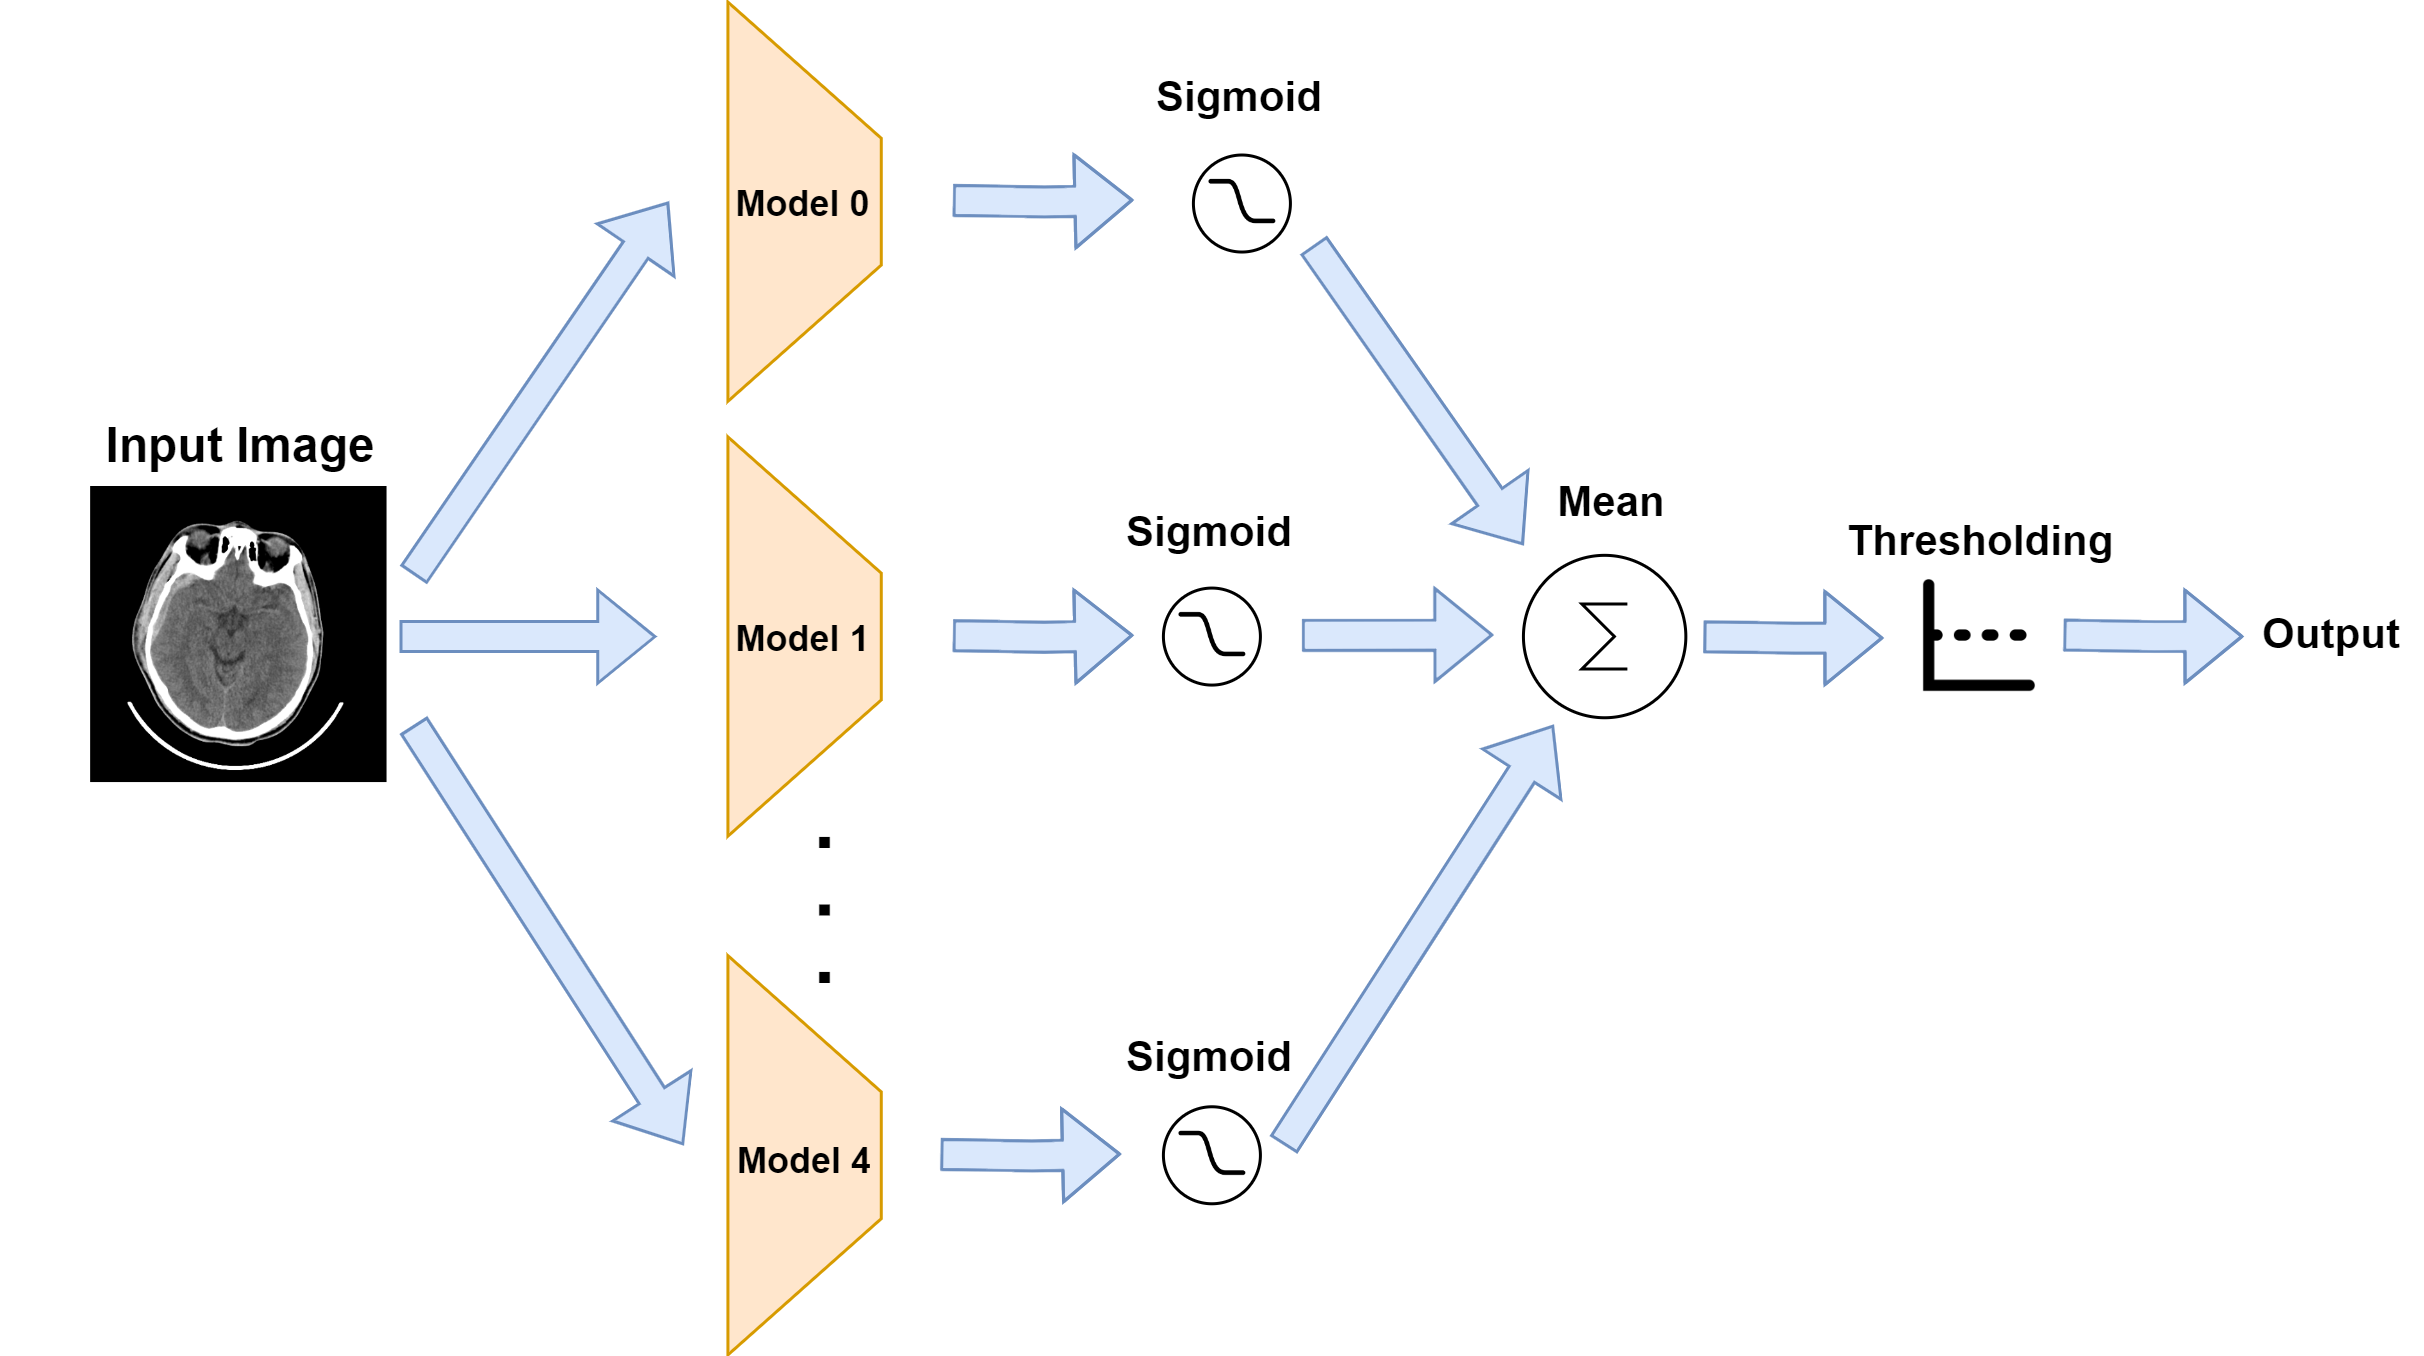
\includegraphics[width=\linewidth]{Images/Chapter2/decision_making.drawio}
			\caption{سازوکار طبقه‌بندی}
			\label{f61}
		\end{subfigure}\hfil % <-- 
		\begin{subfigure}{0.49\textwidth}
			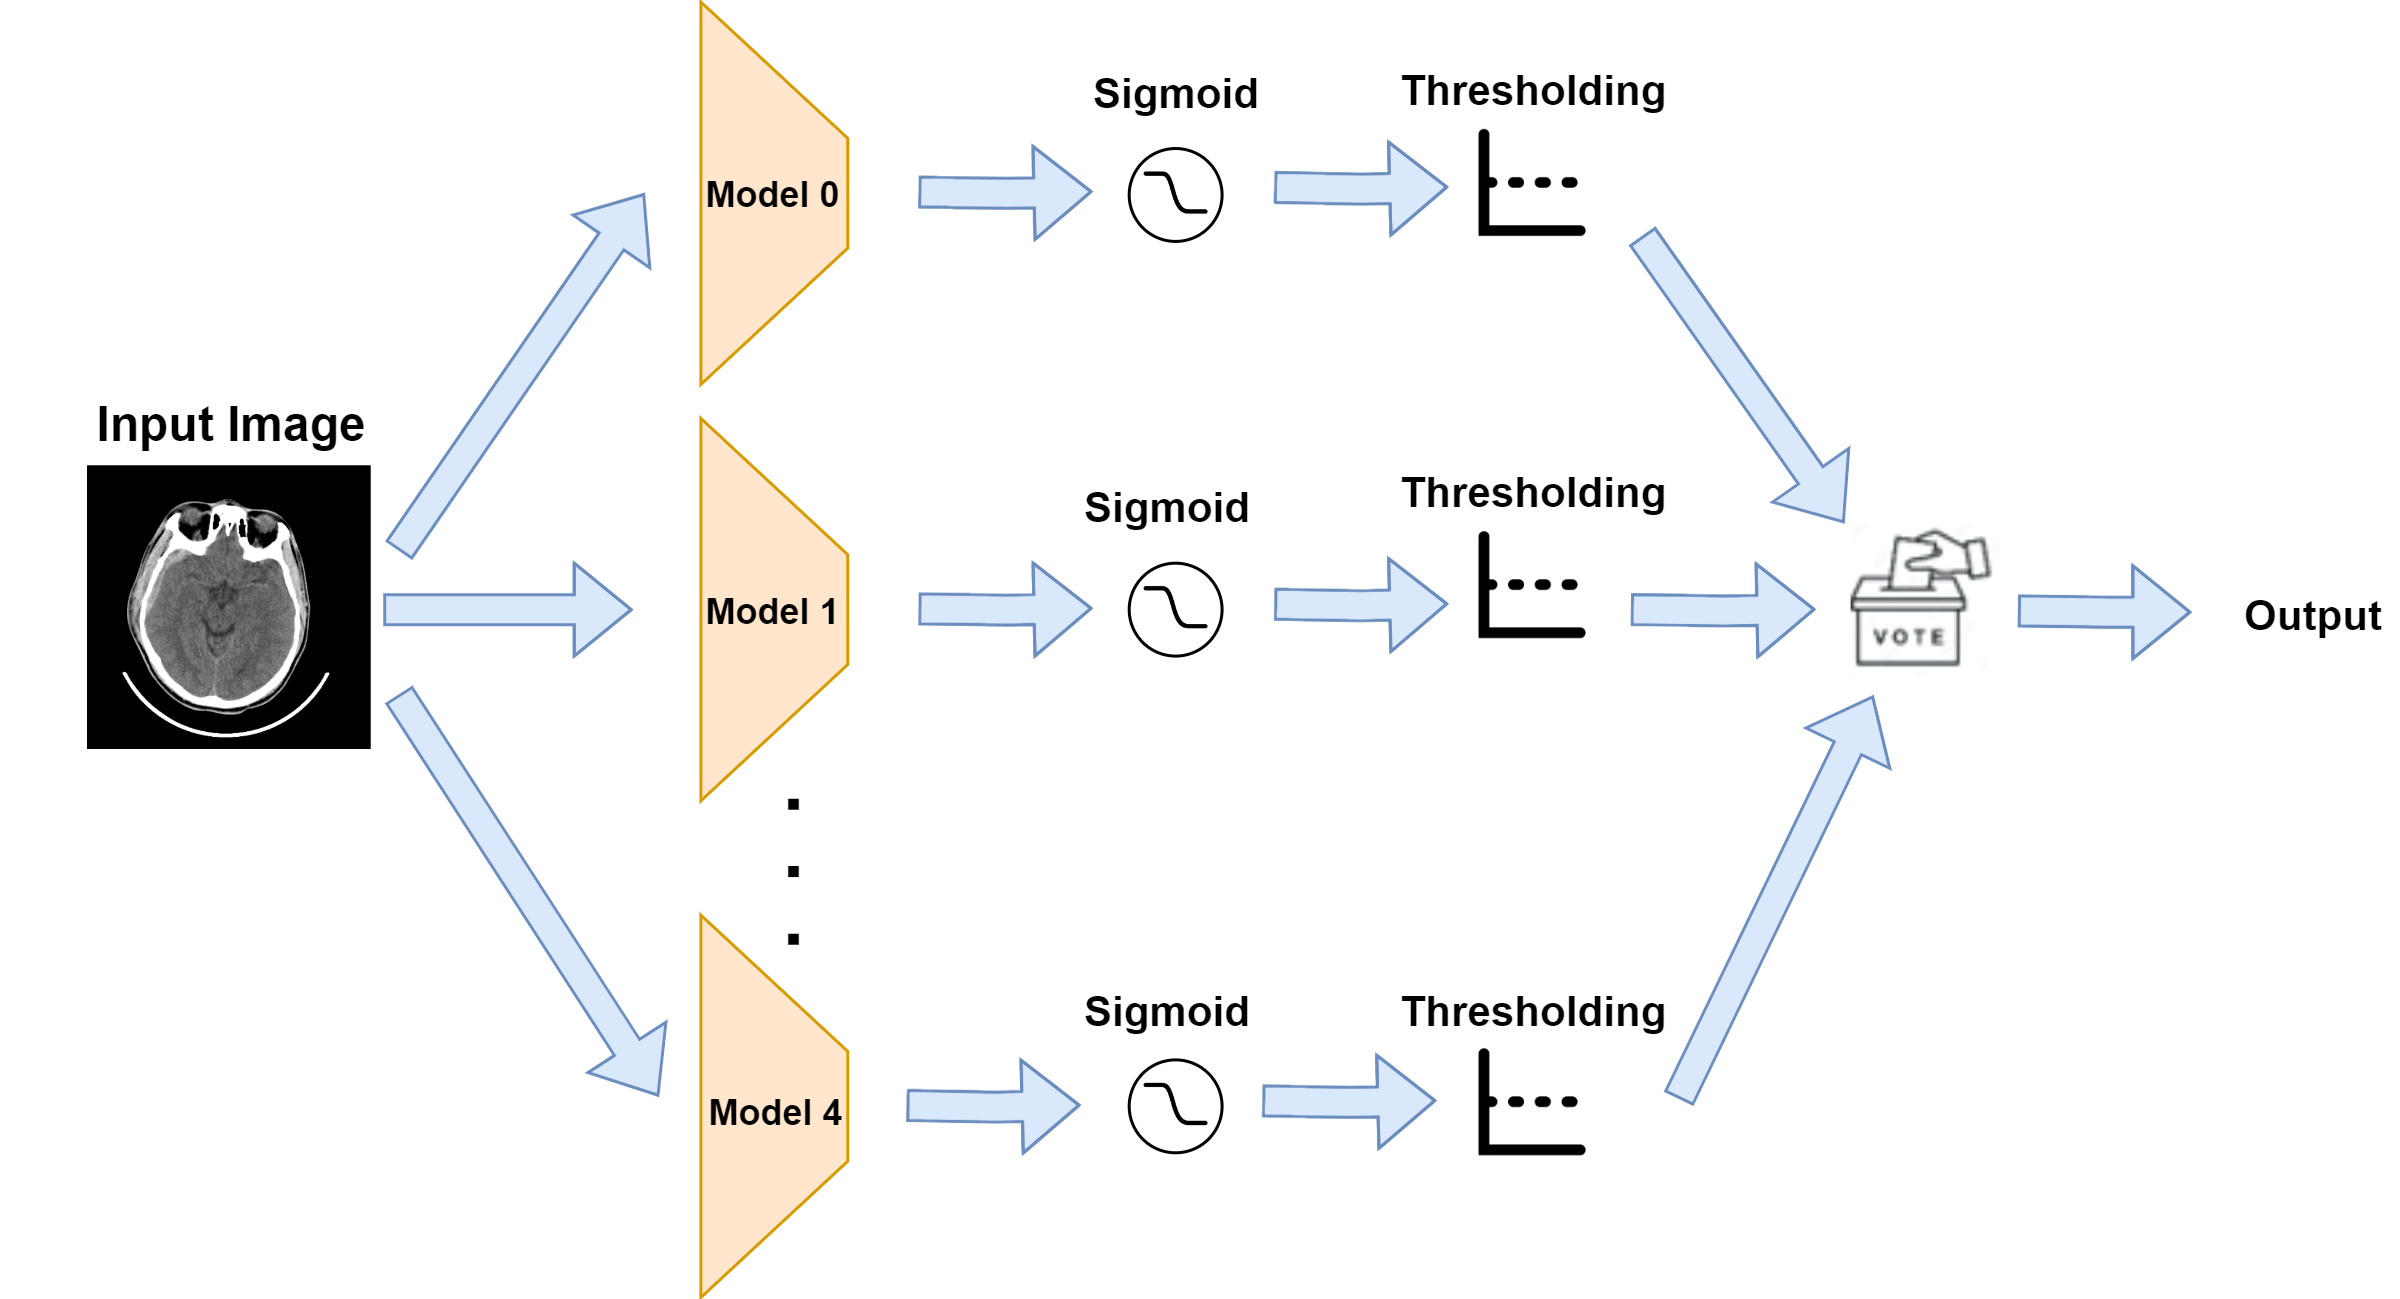
\includegraphics[width=\linewidth]{Images/Chapter2/decision_making_seg.drawio}
			\caption{سازوکار قطعه‌بندی}
			\label{f62}
		\end{subfigure}\hfil % <-- added

		\caption{سازوکار تصمیم‌گیری شورایی}
		\label{fig:decisionmaking}
\end{figure}

